% LaTeX/AMS-LaTeX

\documentclass[a4paper,11pt]{book}

%%% remove comment delimiter ('%') and specify encoding parameter if required,
%%% see TeX documentation for additional info (cp1252-Western,cp1251-Cyrillic)
%\usepackage[cp1252]{inputenc}

%%% remove comment delimiter ('%') and select language if required
%\usepackage[english,spanish]{babel}

\usepackage{amssymb}
\usepackage{amsmath}
\usepackage[dvips]{graphicx}
%%% remove comment delimiter ('%') and specify parameters if required
%\usepackage[dvips]{graphics}

\begin{document}

%%% remove comment delimiter ('%') and select language if required
%\selectlanguage{spanish} 

\noindent 

\noindent 

\noindent 

\noindent 

\noindent 

\noindent 

\noindent 

\noindent 

\noindent 

\noindent 

\noindent 

\noindent 

\noindent 

\noindent 

\noindent 

\noindent 
\includegraphics[bb=0mm 0mm 208mm 296mm, width=16.7mm, height=22.2mm, viewport=3mm 4mm 205mm 292mm]{image12.ps}Perl and Databases

\noindent 

\noindent 

\noindent 

\noindent 

\noindent Building  database applications  is  without  doubt  one  of  the  most  common  uses  of  Perl. With its excellent  support  for interfacing  with  a  very  broad  range  of database  formats,  this  support  comes two guises:

\noindent 

\noindent ? For simpler applications, we've got the DBM (DataBase Manager) modules. DBM is a generic term for a family of simple database formats, they come in several different flavors, and you'll find them in common use, particularly on UNIX platforms. Perl supports all DBM formats through a tied hash, so that the contents of the database look to us just like a normal hash variable.

\noindent 

\noindent ? For more advanced database applications, Perl provides the DataBase Interface (DBI) module.

\noindent DBI is a generic database interface for communicating with database servers that use

\noindent Structured Query Language (SQL) to get at data. To use DBI, we also need to install a

\noindent database driver (DBD) module for the database we want to connect to. These are available for all popular databases, including MySQL, mSQL, Oracle, Informix, and Sybase.

\noindent 

\noindent DBI provides abstraction -- we can write our code without paying too much attention to the database

\noindent that sits behind it all. Meanwhile, the DBD module provides us with all the database-specific parts. By using DBI, we can take the same approach to all our programming, no matter what underlying database we happen to be using.

\noindent 

\noindent \textit{ODBC and remote database access are also available as DBD modules, so any database that supports ODBC can also be accessed by Perl using DBI.}

\noindent 

\noindent In this chapter, we're going to look at how Perl works with both of these. Since DBM is far simpler and requires no database server to be installed and configured, we'll look at it first. We'll then move on to DBI, covering a little basic SQL as we go, and see how we can use it to implement more advanced database applications.

\noindent  

\noindent  

\noindent  

\noindent  

\noindent 

\noindent Perl and DBM

\noindent 

\noindent DBM  databases  have existed on  UNIX  systems  for  many  years,  and  since  Perl  draws  on  a  lot

\noindent of UNIX  history,  it's supported  DBM  databases  virtually  from  day  one.  Once  upon  a  time,  Perl actively  supported dbmopen and  dbmclose functions  for  the  purpose  of  interfacing  with  DBM files,  they still  exist  in the  language,  but  really  only  for  reasons  of  backward  compatibility  with

\noindent older Perl scripts.  In these  enlightened  times,  we  can  use  the  more powerful  (and  infinitely  more convenient) tied  hash interface.

\noindent 

\noindent DBM  databases  can  best be thought  of as  basic  card-file  databases  --  they  support  a  fairly  simple

\noindent form of key-value  association that  translates  easily  into  a  Perl  hash  when  tied.  DBM  does  not  support indexes,  binary trees  (with the  exception  of  Berkeley  DB),  complex  record  structures,  multiple

\noindent tables,  or transactions,  for any  of these  we'll  need  to  use  a  proper  database  server,  most  likely  via

\noindent a  DBI interface.

\noindent 

\noindent Which DBM Implementation To Use

\noindent 

\noindent There are five main DBM implementations, each supported by a C library. Each uses its own file format for the databases it creates (although some libraries, notably GDBM, support the ability to access

\noindent databases created with a different DBM implementation). Since it's entirely possible that your operating

\noindent system has no support for any native DBM format (Windows, for example) Perl provides us with the

\noindent SDBM format as a fall-back option. The five are:

\noindent 

\noindent ? \textbf{gdbm   }-- the GNU DBM database. The fastest and most portable of the standard DBM

\noindent implementations (only Berkeley DB is faster). As well as its own storage format, it can read

\noindent and write NDBM databases. Supports limited file and record locking -- handy for concurrent user access. Freely downloadable under the GNU Public License (from www.gnu.org and almost every FTP repository on the planet).

\noindent 

\noindent ? \textbf{ndbm   }-- the "new" DBM implementation. The version of DBM most commonly found on current UNIX systems. Not as powerful or feature-rich as GDBM, but it's good enough for most purposes if GDBM isn't available.

\noindent 

\noindent ? \textbf{odbm   }-- the "old" DBM implementation. Also known as just "DBM". This is the version of DBM that originally appeared on UNIX systems. It's largely been replaced by NDBM and should be avoided if possible.

\noindent 

\noindent ? \textbf{sdbm   }-- comes as standard with Perl. Not as efficient as the other DBM formats (especially GDBM). It's not well-suited to large databases, but is guaranteed to work anywhere that Perl can be installed, so it's useful for ensuring cross-platform portability.

\noindent 

\noindent ? \textbf{bsd-db   }-- the "Berkeley" DB format. Not strictly a DBM database at all, but it can be considered a close relative and is frequently found on BSD Unix systems. Like GDBM, DB supports file and record locking. More powerful than any of the DBM implementations. Supports a binary tree format as well as DBM's simple hash format -- both can be used by the DBM-like interface provided by Perl. You can get it from http://www.sleepycat.com/.

\noindent 

\noindent Perl can only support a given DBM format if the supporting libraries are actually installed on the

\noindent system. When Perl is built, it scans the system and builds Perl module wrappers for all DBM file formats for which it can find libraries. Therefore, to use GDBM, we must first install the GDBM package (from www.gnu.org and many mirrors) and then Perl itself.

\noindent 

\noindent 

\noindent We'll largely assume the use of SDBM throughout this chapter, but all the examples should also work

\noindent with the other implementations above. Bear in mind that SDBM isn't ideal, so where you have an option, you should probably consider using GDBM. Although most of the following examples specify use SDBM, you can easily adapt them to use any other DBM format by substituting the relevant

\noindent module name.

\noindent 

\noindent And we're on the subject\dots  Say you're running a script that wants to use GDBM, and it   fails because it can't find the Perl module for GDBM support. The chances are, it's not because Perl was installed incorrectly, but simply that you didn't have GDBM handy when Perl was installed. Surely this presents a problem if we're trying to write portable Perl scripts?

\noindent 

\noindent Well, not necessarily. There's one more module we should at least mention, called AnyDBM\_File. It's not actually DBM implementation itself, but as we'll see later on in the chapter, we can use it to avoid having to explicitly specify any particular implementation in our program.

\noindent 

\noindent Accessing DBM Databases

\noindent 

\noindent While the various DBM libraries use different formats internally, the way we access each of them is identical. In the past, we would use the (now obsolete) dbmopen and dbmclose functions to create a connection between our Perl program and a DBM database. These days we use tie to bind our chosen DBM implementation to a hash variable -- we can then manipulate the variable, and in doing so,

\noindent directly modify the data stored in the underlying database file. As we'll see, handling DBM databases from Perl is actually \textit{really easy}.

\noindent 

\noindent \textit{Opening a DBM Database}

\noindent As we mentioned above, DBM databases are accessed by using tie to associate them with a regular hash variable. Once tied, all accesses to the hash are invisibly translated into database reads, and all

\noindent modifications, additions, or deletions are invisibly translated into database writes. This \textbf{tied hash }lets us maintain the database invisibly, just using ordinary Perl statements to manipulate the hash.

\noindent 

\noindent The tie statement for DBM files takes five parameters:

\noindent 

\noindent ? the hash variable to be tied

\noindent 

\noindent ? the DBM module providing the actual database

\noindent 

\noindent ? the name of the database to tie to

\noindent 

\noindent ? the file-access options

\noindent 

\noindent ? the file-access mode

\noindent 

\noindent For now, let's assume we already have a DBM database, demo.dbm -- you can get this sample file as

\noindent part of the book's code download (available from www.wrox.com). Here's how we'd open it up for read-

\noindent write access:

\noindent 

\noindent \#!/usr/bin/perl

\noindent \#opendbm.plx

\noindent use warnings;

\noindent use strict;

\noindent use POSIX;

\noindent use SDBM\_File; \# or GDBM\_File / NDBM\_File / AnyDBM\_File...

\noindent 

\noindent 

\noindent my \%dbm;

\noindent my \$db\_file="demo.dbm";

\noindent 

\noindent tie \%dbm, 'SDBM\_File', \$db\_file, O\_RDWR, 0;

\noindent 

\noindent Most of this is self-explanatory, with the exception of the last two arguments to tie:

\noindent 

\noindent ? O\_RDWR is a symbol imported from the POSIX module, which defines common labels for system values. In this case, we have specified the \textbf{open read-write }flag, telling perl that we want to open the file for both reading and writing.

\noindent 

\noindent ? '0'  specifies the  \textbf{file permissions  }we're  using  to  open  the  database  with.  For now,  this  default value  is fine.  When we start  to  create  databases,  things  become  more  interesting,  as  we'll  see later.

\noindent 

\noindent \textit{Checking the State of a DBM Database}

\noindent Just like any other system call, tie returns a true value if successful, so we should really say:

\noindent 

\noindent tie \%dbm, 'SDBM\_File', \$db\_file, O\_RDWR, 0 or die "Error opening \$db\_file: \$!\textbackslash n";

\noindent 

\noindent Alternatively, we can check that the tie was successful with tied. If the hash is tied, the database was opened successfully. If not, it's because the tie failed and will have returned an error:

\noindent 

\noindent 

\noindent unless (tied \%dbm) \{

\noindent print "Database is not open - cannot continue!\textbackslash n");

\noindent return;

\noindent \} else \{

\noindent \# do stuff

\noindent \}

\noindent 

\noindent It's also possible for tie to return a fatal error if we feed it parameters it doesn't like. We can trap such errors by placing an eval around the tie statement. eval \{ BLOCK \} effectively says "try this out, but it may go wrong, so don't die if it does", any calls to die that originate from within the block won't

\noindent kill the program. Instead, they'll be intercepted and the relevant error message placed in \$@, from where we can access them as normal to provide an error message. All in all, it's a good way to cover yourself if you're undertaking a risky operation. However, it's also inherently unpredictable, and therefore worth taking extra special care with if you do use it:

\noindent 

\noindent 

\noindent eval \{

\noindent tie \%dbm, 'SDBM\_File', \$db\_file, O\_RDWR, 0;

\noindent \};

\noindent 

\noindent if (\$@) \{

\noindent print "Error tieing to \$db\_file: \$@\textbackslash n";

\noindent \} elsif (!tied(\%dbm)) \{

\noindent print "Error opening \$db\_file: \$!\textbackslash n";

\noindent \}

\noindent 

\noindent 

\noindent \textit{Creating DBM Databases}

\noindent If a requested database doesn't exist, then the above example will return a file not found error. We can

\noindent tell perl to create the database (if it doesn't already exist) by adding the O\_CREAT (create) flag, which we can combine with O\_RDWR using a bitwise or:

\noindent 

\noindent tie \%dbm, 'SDBM\_File', \$db\_file, O\_CREAT\textbar O\_RDWR, 0644;

\noindent 

\noindent Because we're potentially creating the file, we specify a file mode in octal; 0644 specifies read and write access for us, but read-only access for other groups and users. Obviously, this only has any real meaning if the underlying operating system understands the concept of users and file permissions, but

\noindent it's worth specifying for portability reasons. For more details on file modes, see Chapter 6, and

\noindent perldoc -f sysopen.

\noindent 

\noindent Finally, here's how we could open a DBM database for read-only access. We could use this in a CGI

\noindent script that's meant to read (but not modify) a database, thus making it more secure:

\noindent 

\noindent tie \%dbm, 'SDBM\_File', \$db\_file, O\_RDONLY, 0;

\noindent 

\noindent \textit{Emptying the Contents of a DBM Database}

\noindent Because the DBM database is represented as a tied hash, we can empty the entire database using a single undef on the hash itself:

\noindent 

\noindent undef \%dbm;

\noindent 

\noindent This wipes out every key in the hash and, along with it, every entry in the underlying DBM. It's a good demonstration of just how important it is to take care with DBM files -- one false move and you've

\noindent wiped out all your data. (You do make backups though, yes? Good. I thought so.)

\noindent 

\noindent \textit{Closing a DBM Database}

\noindent When we've finished with a database, it's good practice to disconnect from it -- break the link between the hash and the file on disk. Just as file handles are automatically closed when a script ends, tied variables are automatically untied. However, it's bad programming practice to rely on this, since we never know how our script might be modified in the future.

\noindent 

\noindent It's simple enough to untie a DBM database -- just use the untie operator:

\noindent 

\noindent untie \%dbm;

\noindent 

\noindent Note that, as with any tied variable, untie will produce warnings if we untie the DBM hash when there are references to it still in existence. See the perltie documentation page for more details.

\noindent 

\noindent \textit{Adding and Modifying DBM Entries}

\noindent Once a DBM database is tied to our hash variable, we can add and modify data in it by simply accessing the hash variable. To create a new entry in an open database that's tied to \$dbm, we simply add a new

\noindent key-value pair to the hash:

\noindent 

\noindent \$dbm\{'newkey'\}="New Value";

\noindent 

\noindent 

\noindent The value must be a scalar. We cannot supply a reference to a hash or list and expect the database to

\noindent store it. Although the database \textit{will }store the reference, it will store it as a string (in the same way that print translates a reference if we try to print it). This string can't be converted back into a reference, and the data that it points to is not stored in the DBM database.

\noindent 

\noindent \textit{Reading DBM Entries}

\noindent Similarly, we read data from a DBM database by accessing the tied hash variable in the normal ways. So

\noindent to read a particular key value we might put:

\noindent 

\noindent my \$value=\$dbm\{'keyname'\};

\noindent 

\noindent To check if a given key exists in the database:

\noindent 

\noindent if (exists \$dbm\{'keyname'\}) \{...\}

\noindent 

\noindent To get a list of all keys in the database:

\noindent 

\noindent my @keys=keys \%dbm;

\noindent 

\noindent To dump a sorted table of all the keys and values in the database:

\noindent 

\noindent foreach (sort keys(\%dbm)) \{

\noindent print "\$\_  =$>$ \$dbm\{\$\_\}\textbackslash n";

\noindent \}

\noindent 

\noindent As the above examples show, we can treat our database almost exactly as if it was an ordinary hash variable -- that's the beauty of tie.

\noindent 

\noindent \textit{Deleting from a DBM Database}

\noindent If we want to remove the key and its associated data entirely, we can use Perl's delete function, just as with an ordinary hash:

\noindent 

\noindent delete \$dbm\{'key'\};

\noindent 

\noindent Normally, delete just removes a key-value pair from a hash. Remember though, if the hash is tied to a

\noindent DBM database, then the database record will be removed as well.

\noindent 

\noindent Try It Out -- A Simple DBM Database

\noindent 

\noindent Let's have a quick look at how we can bring together what we've seen so far. The following program is a

\noindent simple DBM database manipulator, which we can use to store on disk whatever information we like, in the form of key-value pairs:

\noindent 

\noindent \#!/usr/bin/perl

\noindent \#simpledb.plx

\noindent use warnings;

\noindent use strict;

\noindent use POSIX;

\noindent use SDBM\_File; \# or GDBM\_File / NDBM\_File / AnyDBM\_File...

\noindent 

\noindent 

\noindent my \%dbm;

\noindent my \$db\_file = "simpledb.dbm";

\noindent 

\noindent tie \%dbm, 'SDBM\_File', \$db\_file, O\_CREAT\textbar O\_RDWR, 0644;

\noindent 

\noindent if (tied \%dbm) \{

\noindent print "File \$db\_file now open.\textbackslash n";

\noindent \} else \{

\noindent die "Sorry - unable to open \$db\_file\textbackslash n";

\noindent \}

\noindent 

\noindent \$\_  = ""; \# make sure that \$\_  is defined

\noindent 

\noindent until (/\^{}q/i) \{

\noindent 

\noindent print "What would you like to do? ('o' for options): ";

\noindent chomp(\$\_  = $<$STDIN$>$);

\noindent 

\noindent if (\$\_  eq "o") \{ dboptions() \}

\noindent elsif (\$\_  eq "r") \{ readdb() \}

\noindent elsif (\$\_  eq "l") \{ listdb() \}

\noindent elsif (\$\_  eq "w") \{ writedb() \}

\noindent elsif (\$\_  eq "d") \{ deletedb() \}

\noindent elsif (\$\_  eq "x") \{ cleardb() \}

\noindent else \{ print "Sorry, not a recognized option.\textbackslash n"; \}

\noindent \}

\noindent 

\noindent untie \%dbm;

\noindent 

\noindent \#*** Option Subs ***\#

\noindent 

\noindent sub dboptions \{

\noindent print$<$$<$EOF;

\noindent Options available:

\noindent o - view options

\noindent r - read entry

\noindent l - list all entries

\noindent w - write entry

\noindent d - delete entry

\noindent x - delete all entries

\noindent EOF

\noindent \}

\noindent 

\noindent sub readdb \{

\noindent my \$keyname = getkey();

\noindent if (exists \$dbm\{"\$keyname"\}) \{

\noindent print "Element '\$keyname' has value \$dbm\{\$keyname\}";

\noindent \} else \{

\noindent print "Sorry, this element does not exist.\textbackslash n"

\noindent \}

\noindent \}

\noindent 

\noindent sub listdb \{

\noindent foreach (sort keys(\%dbm)) \{

\noindent print "\$\_  =$>$ \$dbm\{\$\_\}\textbackslash n";

\noindent \}

\noindent \}

\noindent 

\noindent 

\noindent sub writedb \{

\noindent my \$keyname = getkey();

\noindent my \$keyval = getval();

\noindent 

\noindent if (exists \$dbm\{\$keyname\}) \{

\noindent print "Sorry, this element already exists.\textbackslash n"

\noindent \} else \{

\noindent \$dbm\{\$keyname\}=\$keyval;

\noindent \}

\noindent \}

\noindent 

\noindent sub deletedb \{

\noindent my \$keyname = getkey();

\noindent if (exists \$dbm\{\$keyname\}) \{

\noindent print "This will delete the entry \$keyname.\textbackslash n";

\noindent delete \$dbm\{\$keyname\} if besure();

\noindent \}

\noindent \}

\noindent 

\noindent sub cleardb \{

\noindent print "This will delete the entire contents of the current database.\textbackslash n";

\noindent undef \%dbm if besure();

\noindent \}

\noindent 

\noindent \#*** Input Subs ***\#

\noindent 

\noindent sub getkey \{

\noindent print "Enter key name of element: ";

\noindent chomp(\$\_  = $<$STDIN$>$);

\noindent \$\_;

\noindent \}

\noindent 

\noindent sub getval \{

\noindent print "Enter value of element: ";

\noindent chomp(\$\_  = $<$STDIN$>$);

\noindent \$\_;

\noindent \}

\noindent 

\noindent sub besure \{

\noindent print "Are you sure you want to do this?";

\noindent \$\_  = $<$STDIN$>$;

\noindent /\^{}y/i;

\noindent \}

\noindent 

\noindent \textit{How It Works}

\noindent Once we've done our usual preliminaries, specifying use POSIX and use SDBM\_File, we declare our hash and specify the filename to use:

\noindent 

\noindent my \%dbm;

\noindent my \$db\_file = "simpledb.dbm";

\noindent 

\noindent Next, we use these values to tie together the hash and the file (creating the file if necessary), confirming success if it works, and telling the program to die otherwise:

\noindent 

\noindent tie \%dbm, 'SDBM\_File', \$db\_file, O\_CREAT\textbar O\_RDWR, 0644;

\noindent 

\noindent if (tied \%dbm) \{

\noindent print "File \$db\_file now open.\textbackslash n";

\noindent \} else \{

\noindent die "Sorry - unable to open \$db\_file\textbackslash n";

\noindent \}

\noindent 

\noindent 

\noindent Now, we set up an until loop. This prompts the user for a standard input and, for specific responses,

\noindent calls appropriate subroutines. The loop continues until \$\_ can be matched to the regular expression

\noindent /\^{}q/i -- in other words, the user enters \textbf{q }or \textbf{Quit }(or, for that matter, \textbf{qwertyuiop}):

\noindent 

\noindent 

\noindent until (/\^{}q/i) \{

\noindent 

\noindent print "What would you like to do? ('o' for options): ";

\noindent chomp(\$\_  = $<$STDIN$>$);

\noindent 

\noindent if (\$\_  eq "o") \{ dboptions() \} elsif (\$\_  eq "r") \{ readdb() \} elsif (\$\_  eq "l") \{ listdb() \} elsif (\$\_  eq "w") \{ writedb() \} elsif (\$\_  eq "d") \{ deletedb() \} elsif (\$\_  eq "x") \{ cleardb() \}

\noindent else \{ print "Sorry, not a recognized option.\textbackslash n"; \}

\noindent \}

\noindent 

\noindent and once we're done with the until loop, we're done with the database -- so we untie from the hash:

\noindent 

\noindent 

\noindent untie \%dbm;

\noindent 

\noindent Now we move on to the subroutines. The first six of these correspond to our six options above. The first displays a list of those options, using a here-document:

\noindent 

\noindent sub dboptions \{

\noindent print$<$$<$EOF;

\noindent Options available:

\noindent o - view options r - read entry

\noindent l - list all entries w - write entry

\noindent d - delete entry

\noindent x - delete all entries

\noindent EOF

\noindent \}

\noindent 

\noindent The second lets the user specify the name of a hash key and displays the corresponding value. That is, unless the key doesn't exist, in which case we offer an explanation:

\noindent 

\noindent sub readdb \{

\noindent my \$keyname = getkey();

\noindent if (exists \$dbm\{"\$keyname"\}) \{

\noindent print "Element '\$keyname' has value \$dbm\{\$keyname\}";

\noindent \} else \{

\noindent print "Sorry, this element does not exist.\textbackslash n"

\noindent \}

\noindent \}

\noindent 

\noindent 

\noindent Next, a variation on the above. This simply lists all the key-value pairs in the database:

\noindent 

\noindent sub listdb \{

\noindent foreach (sort keys(\%dbm)) \{

\noindent print "\$\_  =$>$ \$dbm\{\$\_\}\textbackslash n";

\noindent \}

\noindent \}

\noindent 

\noindent The fourth subroutine lets the user specify both a key and a value, and as long as the key hasn't already

\noindent been used, it uses this pair to define a new entry in the database:

\noindent 

\noindent sub writedb \{

\noindent my \$keyname = getkey();

\noindent my \$keyval = getval();

\noindent 

\noindent if (exists \$dbm\{\$keyname\}) \{

\noindent print "Sorry, this element already exists.\textbackslash n"

\noindent \} else \{

\noindent \$dbm\{\$keyname\}=\$keyval;

\noindent \}

\noindent \}

\noindent 

\noindent Next,  the user  can  specify  a key,  and  (following  a  warning)  the corresponding  entry  in  the  database

\noindent is deleted:

\noindent 

\noindent sub deletedb \{

\noindent my \$keyname = getkey();

\noindent if (exists \$dbm\{\$keyname\}) \{

\noindent print "This will delete the entry \$keyname.\textbackslash n";

\noindent delete \$dbm\{\$keyname\} if besure();

\noindent \}

\noindent \}

\noindent 

\noindent Finally, the cleardb subroutine lets the user wipe the whole database clean:

\noindent 

\noindent sub cleardb \{

\noindent print "This will delete the entire contents of the current database.\textbackslash n";

\noindent undef \%dbm if besure();

\noindent \}

\noindent 

\noindent In several of the subroutines above, we had cause to perform certain checks several times over. Rather than spelling them out for each subroutine, we put them into subroutines of their own, and these are

\noindent what we now come to.

\noindent 

\noindent The first two of these are essentially the same -- both prompt the user for an input, which is chomped and then returned to the calling code:

\noindent 

\noindent sub getkey \{

\noindent print "Enter key name of element: ";

\noindent chomp(\$\_  = $<$STDIN$>$);

\noindent \$\_;

\noindent \}

\noindent 

\noindent 

\noindent Only the text of the prompt differs between the two: one requesting a key, the other a value:

\noindent 

\noindent sub getval \{

\noindent print "Enter value of element: ";

\noindent chomp(\$\_  = $<$STDIN$>$);

\noindent \$\_;

\noindent \}

\noindent 

\noindent The very last subroutine lets us add warnings to potentially dangerous operations -- once again, this will prompt for a user input, but then return TRUE if (and only if) that input matches /\^{}y/i, that is \textbf{y}, \textbf{Yes}

\noindent (or even \textbf{yeah!}):

\noindent 

\noindent sub besure \{

\noindent print "Are you sure you want to do this?";

\noindent \$\_  = $<$STDIN$>$;

\noindent /\^{}y/i;

\noindent \}

\noindent 

\noindent As we saw above, this can be added to operations \textit{very }simply, by saying:

\noindent 

\noindent \textit{$<$do\_something\_risky$>$ }if besure();

\noindent 

\noindent with the result that nothing happens \textit{unless }the user specifically responds 'y'.

\noindent 

\noindent Writing Portable DBM Programs with the AnyDBM Module

\noindent 

\noindent Sometimes we won't care which DBM format we use, just so long as it works. This is particularly true if we want to write a portable script that will work on any system, regardless of which DBM

\noindent implementations it supports. If we want our program to run on someone else's computer, there's no way we can tell in advance what DBM library they have.

\noindent 

\noindent Fortunately, there's a way around this problem. The AnyDBM module is a convenient wrapper around

\noindent all the DBM modules, which can be substituted wherever we'd normally use a specific DBM module. It searches the system for different DBM implementations and uses the first one it finds. By using this, we can avoid having to choose a DBM format and leave it to the script. Here is an example of how we can use AnyDBM to tie to an arbitrary DBM database format:

\noindent 

\noindent 

\noindent \#!/usr/bin/perl

\noindent \#anydbm.plx

\noindent use strict;

\noindent use warnings;

\noindent use AnyDBM\_File;

\noindent use POSIX;

\noindent 

\noindent my \%dbm;

\noindent my \$db\_file="anydbmdemo.dbm";

\noindent 

\noindent tie (\%dbm, 'AnyDBM\_File', \$db\_file, O\_CREAT\textbar O\_RDWR, 0644);

\noindent 

\noindent 

\noindent unless (tied \%dbm) \{

\noindent print "Error opening \$db\_file \$!\textbackslash n";

\noindent \} else \{

\noindent \$dbm\{'Created'\}=localtime;

\noindent foreach (sort keys \%dbm) \{

\noindent print "\$\_  =$>$ \$dbm\{\$\_\}\textbackslash n";

\noindent \}

\noindent untie \%dbm;

\noindent \}

\noindent 

\noindent AnyDBM searches for DBM database implementations in a predefined order, defined by the contents of

\noindent its @ISA array. As we saw in the previous chapter, this is a special array, used to define what parents a child object inherits its methods from. The search will therefore look for modules in the order specified

\noindent by the elements in that array -- this is the default order:

\noindent 

\noindent ? NDBM\_File

\noindent 

\noindent ? DB\_File

\noindent 

\noindent ? GDBM\_File

\noindent 

\noindent ? SDBM\_File

\noindent 

\noindent ? ODBM\_File

\noindent 

\noindent AnyDBM will therefore create an NDBM database in preference to any other kind; failing that, a Berkeley

\noindent (BSD) DB database; then a GDBM database; an SDBM database; and finally, an ODBM database. Since

\noindent SDBM is guaranteed to exist, ODBM will typically never be reached.

\noindent 

\noindent By predefining AnyDBM's @ISA array we can change the order in which it searches the various DBM modules. If we want to tell AnyDBM that we prefer GDBM (which we probably do), with NBDM second and SDBM third, but that we do not want to use ODBM or BSD DB, even if they are installed, we'd write:

\noindent 

\noindent BEGIN \{

\noindent @AnyDBM\_File::ISA = qw(GDBM\_File NDBM\_File SDBM\_File);

\noindent \}

\noindent use AnyDBM\_File;

\noindent 

\noindent Note that this works because  AnyDBM specifically  checks  to  see  if  its @ISA array  has already  been defined  before  setting  it up with  the  default  order.  This  won't  necessarily  be  the case  for other

\noindent Perl modules.

\noindent 

\noindent Copying from One DBM Format to Another

\noindent 

\noindent Because DBM databases are represented through tie as hashes, converting one database format to another is almost disturbingly easy. Say we wanted to convert an NDBM database to the newer GDBM format. Here's how we do it:

\noindent 

\noindent 

\noindent \#!/usr/bin/perl

\noindent \#copydbm.plx

\noindent use warnings;

\noindent use strict;

\noindent use POSIX;

\noindent use NDBM\_File;

\noindent use GDBM\_File;

\noindent 

\noindent my (\%ndbm\_db,\%gdbm\_db);

\noindent my \$ndbm\_file='/tmp/my\_old\_ndbm\_database';

\noindent my \$gdbm\_file='/tmp/my\_new\_gdbm\_database';

\noindent 

\noindent tie \%ndbm\_db, 'NDBM\_File',\$ndbm\_file, O\_RDONLY, 0;

\noindent tie \%gdbm\_db, 'GDBM\_File',\$gdbm\_file, O\_CREAT\textbar O\_WRONLY, 0644;

\noindent 

\noindent \%gdbm\_db=\%ndbm\_db;

\noindent 

\noindent untie \%ndbm\_db;

\noindent untie \%gdbm\_db;

\noindent 

\noindent As the above example shows, the hard part of the conversion is handled for us in a simple hash copy.

\noindent 

\noindent Complex Data Storage

\noindent 

\noindent Now, as we've seen, DBM databases get on just fine with scalar variables, but it seems that's about \textit{all }they can handle. So what if we want to store complex data like lists and hashes? The rough-and-ready answer is we need to convert them into a form that is, scalar string values that DBM \textit{can }store. If we're mainly storing strings of varying sizes, the easiest option is join them with a separator that's guaranteed

\noindent never to occur in the data. For example, to store a list we might use:

\noindent 

\noindent \$dbm\{'key'\}=join ("\_XYZ\_",@list);

\noindent 

\noindent We can subsequently retrieve the packed values with the split function:

\noindent 

\noindent my @list=split "\_XYZ\_",\$dbm\{'key'\};

\noindent 

\noindent However, it turns out we don't actually have to labor over interminable joins and splits, because (surprise, surprise!) we can use one of Perl's \textbf{serializing }modules. These do exactly the same job, but rather more efficiently and flexibly. The three main choices are Data::Dumper, Storable, and FreezeThaw (all of which are available from your nearest CPAN mirror).

\noindent 

\noindent Of the three, Storable is the most flexible, and FreezeThaw the most lightweight. Data::Dumper

\noindent is the oldest, but also the least efficient. Here's an example using Storable's freeze and thaw to store hashes in a DBM file:

\noindent 

\noindent \#!/usr/bin/perl

\noindent \#hashdbm.plx

\noindent use warnings;

\noindent use strict;

\noindent use POSIX;

\noindent 

\noindent 

\noindent use SDBM\_File;

\noindent use Storable;

\noindent 

\noindent my \%dbm;

\noindent my \$db\_file="demo.dbm";

\noindent 

\noindent tie \%dbm, 'SDBM\_File', \$db\_file, O\_CREAT\textbar O\_RDWR, 0644;

\noindent 

\noindent \# store a hash in DBM (note that we must supply a reference):

\noindent \$dbm\{'key'\}=Storable::freeze(\{Name=$>$"John", Value=$>$"Smith", Age=$>$"42"\});

\noindent 

\noindent \# retrieve a hash from DBM (as a reference or as a hash):

\noindent my \$href=Storable::thaw(\$dbm\{'key'\});

\noindent my \%hash=\%\{ Storable::thaw(\$dbm\{'key'\}) \};

\noindent 

\noindent 

\noindent Multi-Level DBM (MLDBM)

\noindent 

\noindent We know that DBM databases only store scalar values -- they won't store lists or hashes unless we take steps to convert them into strings, a process known as \textbf{s}erializing. Fortunately, we don't have to do the

\noindent work of serializing ourselves, since there are several Perl modules that will do it for us -- we just saw how the Storable module can do this.

\noindent 

\noindent However, even \textit{this }is more work than we need to do. There's a module available on CPAN called

\noindent MLDBM, which bundles a DBM module together with a serializing module transparently. This allows us

\noindent to create complex data structures in a DBM file without having to worry about how they're stored. With MLDBM we can store hashes of hashes, lists of lists, hashes of list, and even hashes of lists of hashes. \textit{Any }type of data structure that can be created in Perl can be stored in an MLDBM database.

\noindent 

\noindent Opening an MLDBM database is similar to opening a regular DBM database:

\noindent 

\noindent \#!/usr/bin/perl

\noindent \#mldbm1.plx

\noindent use warnings;

\noindent use strict;

\noindent use MLDBM;

\noindent use POSIX; \#for O\_CREAT and O\_RDWR symbols

\noindent use strict;

\noindent 

\noindent my \%mldbm;

\noindent my \$mldb\_file="mlanydbmdemo.dbm";

\noindent 

\noindent tie \%mldbm, 'MLDBM', \$mldb\_file, O\_CREAT\textbar O\_RDWR, 0644;

\noindent 

\noindent This creates an SDBM database to store the actual data, and uses the Data::Dumper module to do the serializing. Neither of these choices is a particularly good one: SDBM is not great for anything but small databases, and Data::Dumper serializes data as actual Perl code -- great if we want to eval it, but not very efficient in terms of storage.

\noindent 

\noindent MLDBM is agnostic about which actual DBM package and serializer we use, just so long as the functions it requires are supported. Here's an example of using MLDBM to manage a GDBM database with data

\noindent serialized with the Storable module -- a much more efficient solution:

\noindent 

\noindent 

\noindent \#!/usr/bin/perl

\noindent \#mldbm2.plx

\noindent use warnings;

\noindent use strict;

\noindent use GDBM\_File;

\noindent use Storable;

\noindent use MLDBM qw(GDBM\_File Storable);

\noindent use POSIX; \#for O\_CREAT and O\_RDWR symbols

\noindent use strict;

\noindent 

\noindent my \%mldbm;

\noindent my \$mldb\_file="mlanydbmdemo.dbm";

\noindent 

\noindent tie \%mldbm, 'MLDBM', \$mldb\_file, O\_CREAT\textbar O\_RDWR, 0644;

\noindent 

\noindent We can use MLDBM with AnyDBM, too, removing the need to choose the underlying database. Because we've decided to have a preference for GDBM, we'll also alter AnyDBM's search order:

\noindent 

\noindent \#!/usr/bin/perl

\noindent \#mldbm3.plx

\noindent use warnings;

\noindent use strict;

\noindent BEGIN \{

\noindent @AnyDBM\_File::ISA = qw(GDBM\_File DB\_File NDBM\_File SDBM\_File);

\noindent \}

\noindent 

\noindent use AnyDBM\_File;

\noindent use Storable;

\noindent use MLDBM qw(AnyDBM\_File Storable);

\noindent use POSIX; \#for O\_CREAT and O\_RDWR symbols

\noindent use strict;

\noindent 

\noindent my \%mldbm;

\noindent my \$mldb\_file="mlanydbmdemo.dbm";

\noindent 

\noindent tie (\%mldbm, 'MLDBM', \$mldb\_file, O\_CREAT\textbar O\_RDWR, 0644);

\noindent 

\noindent unless (tied \%mldbm) \{

\noindent print "Error opening \$mldb\_file: \$!\textbackslash n";

\noindent \} else \{

\noindent if (exists \$mldbm\{'Created'\}) \{

\noindent \$mldbm\{'Created'\}=localtime;

\noindent \} else \{

\noindent \$mldbm\{'Updated'\}=localtime;

\noindent \}

\noindent foreach (sort keys \%mldbm) \{

\noindent print "\$\_  =$>$ \$mldbm\{\$\_\}\textbackslash n";

\noindent \}

\noindent untie \%mldbm;

\noindent \}

\noindent 

\noindent Once a DBM database has been opened or created via MLDBM, we can modify its contents as before, but

\noindent we're no longer limited to storing scalar values.

\noindent 

\noindent 

\noindent To  finish off our  discussion of  DBM  databases,  we'll  take  a  look  at  program  that  creates  an  MLDBM

\noindent database and writes various kinds  of  values  into  it.  All  the  assignments  below  are valid,  but  note the comments:

\noindent 

\noindent \#!/usr/bin/perl

\noindent \#mldbm4.plx

\noindent use MLDBM qw(SDBM\_File Storable);

\noindent use POSIX;

\noindent use warnings;

\noindent use strict;

\noindent 

\noindent my \%mldbm;

\noindent my \$mldb\_file="mldbmdemo.dbm";

\noindent 

\noindent tie (\%mldbm, 'MLDBM', \$mldb\_file, O\_CREAT\textbar O\_RDWR, 0644);

\noindent 

\noindent unless (tied \%mldbm) \{

\noindent print "Error opening \$mldb\_file: \$!\textbackslash n";

\noindent \} else \{

\noindent \# wipe out the old contents, if any

\noindent undef \%mldbm;

\noindent 

\noindent \$mldbm\{'Created'\}=localtime;

\noindent 

\noindent \# assign a list anonymously, directly and as a copy

\noindent \$mldbm\{'AnonymousList'\}=[1,2,3,4,"Five",6,7.8];

\noindent my @list=(9,"Ten",11,12.13,14);

\noindent \$mldbm\{'OriginalList'\}=\textbackslash @list;

\noindent \$mldbm\{'CopyOfList'\}=[ @list ];

\noindent \$mldbm\{'NumberOfListElems'\}=@list;

\noindent \$list[0]="Nine"; \#does NOT modify 'OriginalList'

\noindent 

\noindent \# assign a hash anonymously, directly and as a copy

\noindent \$mldbm\{'AnonymousHash'\}=\{One=$>$'1',Two=$>$'2',Three=$>$'3'\};

\noindent my \%hash=(Four=$>$'4',Five=$>$'5',Six=$>$'6');

\noindent \$mldbm\{'OriginalHash'\}=\textbackslash \%hash;

\noindent \$mldbm\{'CopyOfHash'\}=\{ \%hash \};

\noindent \$mldbm\{'NumberOfHashKeys'\}=keys \%hash;

\noindent \$hash\{Four\}="IV"; \#does NOT modify 'OriginalHash'

\noindent 

\noindent \# assign a random key and value

\noindent \$mldbm\{rand()\}=rand;

\noindent 

\noindent \# a more complex assignment

\noindent \$mldbm\{'HashOfMixedValues'\}=\{

\noindent List1=$>$[1,2,3],

\noindent List2=$>$[4,5,6],

\noindent String=$>$"A String",

\noindent Hash1=$>$\{

\noindent A=$>$"a",

\noindent B=$>$"b",

\noindent Hash2=$>$\{

\noindent C=$>$"c",

\noindent \},

\noindent \},

\noindent Number=$>$14.767,

\noindent List3=$>$[7,8,9],

\noindent \};

\noindent 

\noindent 

\noindent \# now dump out the contents again

\noindent foreach (sort keys \%mldbm) \{

\noindent print "\$\_  =$>$ \$mldbm\{\$\_\}\textbackslash n";

\noindent if (my \$ref=ref \$mldbm\{\$\_\}) \{

\noindent if (\$ref eq 'HASH') \{

\noindent foreach my \$key (sort keys \%\{ \$mldbm\{\$\_\} \})\{ 

\noindent print "\textbackslash t\$key =$>$ \$mldbm\{\$\_\}\{\$key\}\textbackslash n";

\noindent \}

\noindent \} else \{

\noindent print "\textbackslash t",(join ",",@\{ \$mldbm\{\$\_\} \}),"\textbackslash n";

\noindent \}

\noindent \}

\noindent \}

\noindent 

\noindent untie \%mldbm;

\noindent \}

\noindent 

\noindent There are three main points to note about this example:

\noindent 

\noindent ? We can assign an existing hash or list either:

\noindent ? with a backslash reference to the original,

\noindent ? or with a reference constructor (using curly or square brackets).

\noindent In both cases, MLDBM makes a \textbf{copy }of the variable. If we try using a backslash reference to point to the original variable, and then change it, the change isn't reflected in the database.

\noindent 

\noindent ? Similarly, if we try taking a reference to anything in a MLDBM database and use it later, it won't work. The reference isn't tied, so it won't be handled by the MLDBM module. We can \textit{only}

\noindent access values through the \textbf{top }of the data structure, where the tie is.

\noindent 

\noindent ? Finally, just as with a normal list, if we don't supply a reference for a value, then we get the number of elements instead -- probably not what we intended.

\noindent 

\noindent 

\noindent Beyond Flat Files and DBM

\noindent 

\noindent There's real power to be had when we're dealing with huge quantities of data in all shapes and sizes. It's enough to take your breath away. The trouble is that so far, we've only really looked at kindergarten-

\noindent level data stores -- while working with DBM is great for speedy solutions, a real-world application of any great size needs to work with a good, powerful, reliable database server.

\noindent 

\noindent Flat files are very simple to work with: They're in an easy-to-read format, even in a simple text editor, and (as long as they're small enough) you can pass on your files around on a floppy disk, should you

\noindent need to use your data on another machine. Unfortunately, it's what they are \textit{not }that's the problem. Our

\noindent .dbm files are essentially text files, so:

\noindent 

\noindent ? Text files aren't scalable. When you search them, each key-value pair in the file is searched sequentially. Consequently, the bigger the file, the more time it's going to take to find what you're looking for.

\noindent ? Cross-referencing data between files is tricky and gets more and more perplexing the greater the number of tables you add into the mix.

\noindent ? It's unwise to give multiple users simultaneous access -- if you let them work on the same data

\noindent at the same time, your files could end up containing inconsistencies.

\noindent 

\noindent 

\noindent There's no easy solution to these problems, at least no set-up that will make everything as easy as

\noindent working with flat files. However, we do at least have the technology to address these problems and make for workable solutions -- we can store our information in \textbf{relational databases}.

\noindent 

\noindent Introducing Relational Databases

\noindent 

\noindent The relational database model was first devised in 1970 and has since developed to a point where practically every major database server -- SQL Server, Oracle, Sybase, DB2, Informix, uses it to store

\noindent data. In this model, items of data are stored in \textbf{tables}, which group together \textbf{records }containing the same

\noindent type of information. So, for example, there might be a record for each patient in a doctor's waiting

\noindent rooms. The database would hold details such as name, address, previous ailments, date of previous visit, and prescriptions stored in separate \textbf{fields}.

\noindent 

\noindent You'd want to hold the same sort of details for every patient, but each set would be specific to a certain one. Each record would therefore require a unique identifier, known as a \textbf{key}, corresponding to one particular patient. This key could then be used to cross-reference information stored in other tables in

\noindent the same database.

\noindent 

\noindent Nowadays, most database vendors following this model also use a similarly generic way to \textbf{query }the database so as to retrieve information. This method takes the form of a language for creating queries to the database -- asking questions if you like. This is called \textbf{Structured Query Language}, or by its more

\noindent familiar name \textbf{SQL }(pronounced 'sequel'). We'll come back to this in a bit, but now, suffice it to say that

\noindent the way in which we write SQL queries remains the same, no matter what database you're querying.

\noindent 

\noindent RDBMS (or Relational DataBase Management Servers, to use their full title) work in quite a different fashion from flat files. Perhaps most notable is the actual lack of a file corresponding to your data.

\noindent Instead, the database server (from now on, just called the 'server') holds all the info within itself, and as

\noindent a rule, viewing the data externally isn't possible, save through querying the server first.

\noindent 

\noindent You may also find it strange to realize that in order to query a database, the server needn't be located on your machine, although in the wonderful world of the Internet, that might not be such a shock. Indeed

\noindent in general, the larger the database and the more data it contains, the more likely it is that the server will be accessed remotely.

\noindent 

\noindent 

\noindent Introducing DBI

\noindent 

\noindent So, relational databases are pretty great -- they do things that flat files and DBM can't, we can ask them questions using the same SQL queries no matter which actual database we're using. So what's the catch? Well, it's a matter of delivering that query to the database and getting back the data we want.

\noindent 

\noindent Technically speaking, it's because each server has a different API (Application Programming Interface) and therefore a different set of commands for doing the same things. Somewhat less technically, it's because behind the scenes, each database uses a different language to talks about the same things.

\noindent 

\noindent When we looked at DBM  files,  there  were  five  different  modules  for the  five  types  of  file we  could

\noindent use.  In the same way,  there's  a  \textbf{database driver  }or  \textbf{DBD }module  for each  type  of  database  server.  So

\noindent if  you  want to  work with a database  on the  Sybase  platform,  you'd  install  the DBD::Sybase module

\noindent and use  it to  query your databases  in  Sybase  language  only.  You  can  see  how  this  can  quickly  become rather a  pain if you're working  with  more  than  one  brand  of  database  and want  to  port  your code between them.

\noindent 

\noindent 

\noindent Enter DBI and your solution. \textbf{DBI }(the standard \textbf{DataBase Interface})  is a database-independent interface

\noindent that sits on top of all these database drivers and acts as a translator for you. All we need do is tell DBI

\noindent 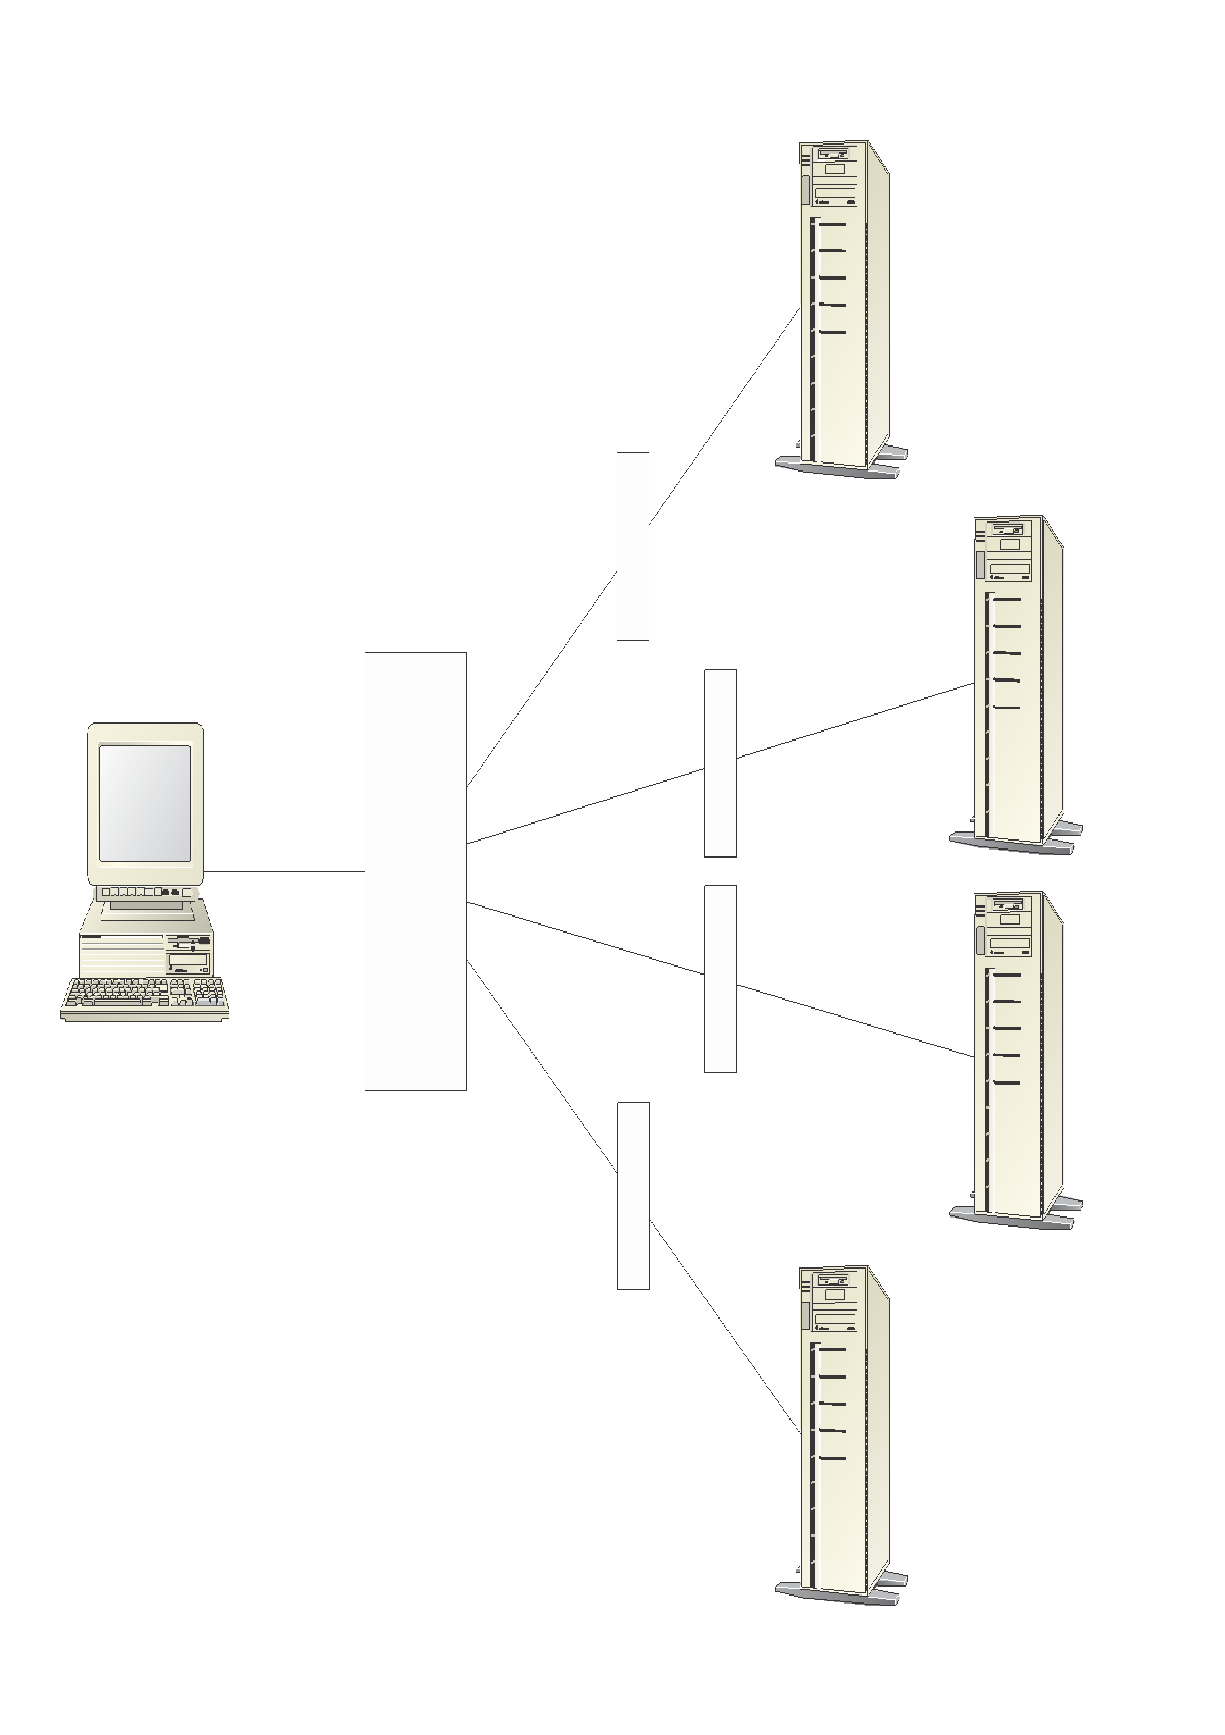
\includegraphics[bb=0mm 0mm 208mm 296mm, width=116.5mm, height=99.3mm, viewport=3mm 4mm 205mm 292mm]{image13.ps}which driver we're using, and it will translate your instructions into those that the driver can understand:

\noindent 

\noindent 

\noindent 

\noindent 

\noindent 

\noindent 

\noindent 

\noindent 

\noindent 

\noindent 

\noindent 

\noindent 

\noindent 

\noindent 

\noindent DBI

\noindent 

\noindent 

\noindent Through our

\noindent computer, we talk to DBI...

\noindent 

\noindent 

\noindent 

\noindent ...which then translates our

\noindent instructions to something the drives can understand and vice  versa.

\noindent 

\noindent 

\noindent 

\noindent The real beauty of DBI is that, if for some reason you come to the conclusion that, say, MySQL isn't offering you the facilities of one of the more high-end databases (like DB2 or Sybase), all you have to do

\noindent is transfer your data to the new DB and redirect your code to look at it -- you won't have to rewrite your code at all.

\noindent 

\noindent So What Do We Need?

\noindent 

\noindent Before going any further,  we  should  find  out what  we  already  have  installed.  We've  already

\noindent established a  rough  shopping  list.  We'll  need  a  database,  a  driver  for  that  database  and DBI  too  -- let's start off with DBI.

\noindent 

\noindent If you're coming to this subject for the first time, the chances are you've not got DBI installed yet, but you can do a simple check by typing perldoc DBI at the command prompt. If it has been installed,

\noindent you'll see:

\noindent 

\noindent $>$\textbf{perldoc DBI}

\noindent NAME

\noindent DBI - Database independent interface for Perl

\noindent 

\noindent SYNOPSIS

\noindent ...

\noindent 

\noindent 

\noindent and so on. On the other hand, if it hasn't been installed yet, you'll get

\noindent 

\noindent $>$\textbf{perldoc DBI}

\noindent No documentation found for "DBI".

\noindent $>$

\noindent 

\noindent If you get this, you'll need to do the obvious and get it up and running. Here's how.

\noindent 

\noindent \textit{Installing DBI}

\noindent DBI is a module just like any other, and can be installed in the same ways we saw in Chapter 10.

\noindent 

\noindent \textit{Installing with PPM}

\noindent Once again, you probably have it easiest if you've installed ActiveState Perl and now have PPM at your disposal. If you're a PPM user, installing DBI is a matter of activating PPM on the command prompt

\noindent and issuing the command:

\noindent 

\noindent $>$\textbf{install DBI}

\noindent 

\noindent The rest of the installation is automatic.

\noindent 

\noindent \textit{Installing from the Source}

\noindent The latest version of the DBI module source code is always available at http://www.symbolstone.org/technology/perl/DBI/. At time of writing, this was at version 1.13. Download the zipped source code and decompress it with Winzip (on Windows) or the command:

\noindent 

\noindent $>$\textbf{gzip -dc DBI-1.13.tar.gz \textbar  tar -xvf}

\noindent 

\noindent We now need to issue the following four commands to compile the source and install our module:

\noindent 

\noindent $>$\textbf{perl makefile.pl}

\noindent $>$\textbf{make}

\noindent $>$\textbf{make test}

\noindent $>$\textbf{make install}

\noindent 

\noindent \textit{Installing from CPAN}

\noindent The last option here is to use the CPAN exporter module and install DBI directly from CPAN. From the command prompt then, there are two simple steps:

\noindent 

\noindent $>$\textbf{perl -MCPAN -e shell}

\noindent cpan$>$ \textbf{install DBI}

\noindent 

\noindent and don't forget to \textbf{quit }CPAN when it's done.

\noindent 

\noindent Try It Out - Quizzing the Drivers

\noindent Now that we're all on a level playing field with DBI installed, let's have a look and see what we get in the base installation that we can use. The following program will do just that for us.

\noindent 

\noindent \#!/usr/bin/perl

\noindent \#available.plx

\noindent use warnings;

\noindent use strict;

\noindent use DBI;

\noindent 

\noindent 

\noindent print "Available DBI Drivers and Data Sources:\textbackslash n\textbackslash n";

\noindent my @drivers=DBI-$>$available\_drivers('quiet');

\noindent my @sources;

\noindent 

\noindent foreach my \$driver (@drivers) \{

\noindent print "\$driver\textbackslash n";

\noindent @sources=eval \{ DBI-$>$data\_sources(\$driver) \};

\noindent if (\$@) \{

\noindent print "\textbackslash tError: ",substr(\$@,0,60),"\textbackslash n";

\noindent \} elsif (@sources) \{

\noindent foreach (@sources) \{

\noindent print "\textbackslash t\$\_\textbackslash n";

\noindent \}

\noindent \} else \{

\noindent print "\textbackslash tNo known data sources\textbackslash n";

\noindent \}

\noindent \}

\noindent 

\noindent With any luck, you'll see the following after a new installation of DBI:

\noindent 

\noindent $>$\textbf{perl available.plx}

\noindent Available DBI Drivers and Data Sources:

\noindent 

\noindent ADO

\noindent 

\noindent No known data sources

\noindent ExampleP

dbi:ExampleP:dir=. Proxy

\noindent Error: install\_driver(Proxy) failed: Can't locate RPC/PlClient.pm ...

\noindent $>$

\noindent 

\noindent We can see then that DBI comes ready with three supplied drivers -- ADO, Proxy, and ExampleP. We'll return in just a short while to see what ADO and Proxy are exactly, when we look at all the

\noindent possible DBDs you can download. However, it's worth noting now that ExampleP is an example DBD

\noindent 'stub' for developers of DBI drivers to work from and provides no useful functionality: that's why it won't be mentioned later.

\noindent 

\noindent \textit{How It Works}

\noindent After the usual headers, the first thing we do is to import the methods that DBI has to offer and then print out a header for our results:

\noindent 

\noindent use DBI;

\noindent 

\noindent print "Available DBI Drivers and Data Sources:\textbackslash n\textbackslash n";

\noindent 

\noindent Now we get to grips with our first DBI method: available\_drivers() simply searches through the directories listed in your @INC array, and if it finds any DBD::* modules, stores them away in

\noindent @drivers:

\noindent 

\noindent my @drivers=DBI-$>$available\_drivers('quiet');

\noindent my @sources;

\noindent 

\noindent 

\noindent Now we simply loop through the drivers we've found and see which databases we can talk to with them:

\noindent 

\noindent foreach my \$driver (@drivers) \{

\noindent print "\$driver\textbackslash n";

\noindent 

\noindent Another DBI method, data\_sources() returns a list of data stores we can talk to through the driver. Note that while it should work fine by itself, we've wrapped our call in an eval clause in case a DBD fails to load. If you remember, eval runs the code under its auspices, but ignores any warnings or calls

\noindent to die from within, which might occur here if the driver fails to install:

\noindent 

\noindent @sources=eval \{ DBI-$>$data\_sources(\$driver) \};

\noindent 

\noindent If an error does occur within eval(), it will get stored in \$@, so we'll print that first. If there isn't one, we either print the data stores we've found that correspond to the driver, or a nice message saying we couldn't find any:

\noindent 

\noindent if (\$@) \{

\noindent print "\textbackslash tError: ",substr(\$@,0,60),"\textbackslash n";

\noindent \} elsif (@sources) \{

\noindent foreach (@sources) \{

\noindent print "\textbackslash t\$\_\textbackslash n";

\noindent \}

\noindent \} else \{

\noindent print "\textbackslash tNo known data sources\textbackslash n";

\noindent \}

\noindent \}

\noindent 

\noindent \textit{What's Available}

\noindent So DBI installs two drivers for future use plus an example one -- there are plenty more out there though, enough to let us work with pretty much any database we choose. Most DBD modules are simply drivers

\noindent for specific third-party database servers (such as Oracle, MySQL, or Informix), but some are in fact interfaces to other database connectivity protocols (such as DBD::ADO and DBD::ODBC), allowing Perl

\noindent to communicate with servers that support these protocols. Programmers wanting to access Microsoft

\noindent SQL servers therefore have both ADO and ODBC (as well as the DBD::Sybase module) as options.

\noindent 

\noindent \textit{A few DBD modules do }not \textit{require a database server. Notable amongst these is the DBD::CSV driver, which makes use of several other Perl modules to provide a SQL interface to database files in comma-separated values (CSV) format. It's a very convenient way to implement a SQL database}

\noindent \textit{with no additional software -- it's also a good way to build prototype database applications before migrating them to a real database server. DBI allows us to write generic code without worrying about the underlying server, so migrating from one database to another shouldn't be a problem.}

\noindent 

\noindent Here's a list of currently supported databases and their DBD modules, all of which are accessible from the Perl DBI homepages at http://www.symbolstone.org/technology/perl/DBI/:

\noindent 

\noindent ? DBD::ADO

\noindent The interface to Microsoft's \textbf{Active Data Objects }data access technology. The driver itself is

\noindent installed with DBI, but in order to pass requests, you'll also need ADO (version 2.1 or later) and the Win32::OLE module installed as well. You can find more about ADO at http://www.microsoft.com/data/ado/.

\noindent 

\noindent 

\noindent ? DBD::Adabas

\noindent The driver for \textbf{Adabase }database servers.

\noindent 

\noindent ? DBD::Altera

\noindent The driver for \textbf{Altera }database servers.

\noindent 

\noindent ? DBD::CSV

\noindent The driver to access Comma-Separated Value files. These files can survive outside and so

\noindent don't require a running database server. This makes them a good choice for creating simple

\noindent SQL-driven databases with a view to migrating to a proper server later on. In addition to

\noindent DBD::CSV however, you'll also need to install the Text::CSV\_XS modules to read and write

\noindent to CSV files and also the SQL::Statement module to parse SQL statements and emulate a real SQL server.

\noindent 

\noindent ? DBD::DB2

\noindent The driver for \textbf{DB2 }database servers, as built by IBM. See

\noindent http://www.softwate.ibm.com/data/db2 for more information.

\noindent 

\noindent ? DBD::Empress

\noindent The driver for \textbf{Empress }database servers and EmpressNet distributed databases. See

\noindent http://www.empress.com for more information.

\noindent 

\noindent ? DBD::Illustra

\noindent The driver for \textbf{Illustra }database servers.

\noindent 

\noindent ? DBD::Informix

\noindent The driver for \textbf{Informix Online }and \textbf{Informix SE }database servers from version 5 onwards.

\noindent Note that in order to work, this driver requires the presence of a licensed copy of the Informix

\noindent Client SDK prior to installation. See http://www.informix.com for more information.

\noindent 

\noindent ? DBD::Ingres

\noindent The driver for Computer Associates' \textbf{Ingres 6.4 }and \textbf{OpenIngres }(all versions) database servers.

\noindent See http://www.cai.com/products/ingres.htm for more information.

\noindent 

\noindent ? DBD::Interbase

\noindent The driver for \textbf{Interbase  }database  servers.  See  http://www.interbase.com  for  more

\noindent information.

\noindent 

\noindent ? DBD::ODBC

\noindent The driver for Microsoft's \textbf{ODBC }database connectivity protocol, versions 2 and 3 on Win32

\noindent and Unix systems. Note that in order for this driver to access a database through ODBC, an underlying ODBC driver for the chosen platform and database is also required. See http://www.microsoft.com/data/odbc for more information.

\noindent ? DBD::Oracle

\noindent The driver for \textbf{Oracle 7 }and \textbf{Oracle 8/8i }database servers. It also includes an emulation mode

\noindent for older 'legacy' Perl scripts written to use the Perl 4 oraperl library. See

\noindent http://www.oracle.com for more information.

\noindent 

\noindent ? DBD::Pg

\noindent The driver for \textbf{PostgreSQL 6.4 }and \textbf{6.5 }databases. This is a freely available open source

\noindent database, frequently bundled with open source operating systems like Linux. See

\noindent http://www.postgresql.org for more information.

\noindent 

\noindent ? DBD::Proxy

\noindent The driver for communicating with \textbf{remote }DBI applications. However, it is not needed to

\noindent access remote databases whose drivers already support remote access. It is useful though for propagating DBI requests through firewalls and can optionally cache networked DBI connections for CGI scripts. DBD::Proxy is bundled with the DBI package itself.

\noindent 

\noindent 

\noindent ? DBD::SearchServer

\noindent The driver for Fulcrum \textbf{SearchServer}/\textbf{PCDOCS}.  See http://www.pcdocs.com for more

\noindent information.

\noindent ? DBD::Solid

\noindent The driver for \textbf{Solid }database servers.

\noindent ? DBD::Sybase

\noindent The driver for \textbf{Sybase 10 }and \textbf{Sybase 11 }database servers. It also has a limited interaction with

\noindent Sybase 4. Interstingly, with the addition of Sybase Open Client or the FreeTDS libraries, this driver can also support Microsoft MS-SQL servers. See http://www.sybase.com, http://www.freetds.org for more information

\noindent ? DBD::Unify

\noindent The driver for \textbf{Unify }database servers.

\noindent ? DBD::XBase

\noindent Contains drivers for \textbf{dBaseIII}, \textbf{dBaseIV}, and \textbf{Fox }databases.

\noindent ? Msql-MySQL-modules

\noindent A  bundle of modules for \textbf{Msql  }and  \textbf{MySQL  }databases,  both  popular  and  freely  available,

\noindent and very similar  in ability.  Includes  the  DBD::mSQL and  DBD::mysql modules.  For more information,  see http://www.Hughes.com.au/products/msql/ and http://www.mysql.com/ respectively.

\noindent 

\noindent While all these modules work similarly and present the same basic interface to DBI, there are many subtle variations in the way that they work. It pays to read the included documentation for a given driver before using it -- perldoc DBD::$<$DriverName$>$ should produce some useful information.

\noindent 

\noindent Our DB of Choice -- MySQL

\noindent 

\noindent For the rest of this chapter, we're going to be working with one specific database and its driver -- MySQL. Why this one in particular? A number of reasons actually:

\noindent 

\noindent ? It's available on the same platforms that DBI is - Solaris, Linux and Windows.

\noindent 

\noindent ? It's fast enough to be run on almost any machine available at the moment.

\noindent 

\noindent ? It's free!

\noindent 

\noindent 

\noindent You can of course choose to follow the rest of this chapter using another database driver. It would be

\noindent quite understandable, for instance, if Windows users decided it best to use DBD::ADO so that they could work with already installed Access or SQL Server databases. The rest of this chapter won't even \textit{try }to teach you everything -- it will however teach you the basics of working with database servers, and will apply to any database you may happen to use. That said, let's get on and get MySQL up and running.

\noindent 

\noindent \textit{Note that if you do decide to use a different database than MySQL, each driver comes with its own}

\noindent \textit{set of methods on top of those in DBI. For example, in this chapter, we briefly use NAME and NUM\_OF\_FIELDS at the end of the chapter that are MySQL specific. Always check the drivers documentation for which methods they do and do not support beside those in DBI}

\noindent 

\noindent 

\noindent \textit{Installing on Windows}

\noindent As usual, installing MySQL on Windows will be a lot simpler than installing it on Linux. You can download the shareware version of MySQL 3.22.34 from the MySQL homepage at http://www.mysql.com. It should come to you as a zipped file -- mysql-shareware-3.22.34- win.zip. If you unzip that, you'll find a file called setup.exe which you should run. The standard installation wizard will run you through a couple of questions. The defaults (a Typical install in C:\textbackslash MySQL) will do fine.

\noindent 

\noindent Once the server and clients have installed, we'll need to get the server itself up and running. Windows

\noindent 95 users should note that MySQL uses TCP/IP to talk to the client, so you'll need to install that from your Windows CD and to download Winsock 2 from the Microsoft website.

\noindent 

\noindent To start MySQL running, you'll need to open a command prompt window, navigate to

\noindent C:\textbackslash MySQL\textbackslash bin, and issue the following command:

\noindent 

\noindent $>$\textbf{mysqld-shareware}

\noindent 

\noindent Likewise, use the following command to shut it down:

\noindent 

\noindent $>$\textbf{mysqladmin -u root shutdown}

\noindent 

\noindent Windows  NT/2000 users also  have  the  option  of running  MySQL  as  a  service.  First  though,  you'll need to  copy and  rename my-example from  C:\textbackslash MySQL to  C:\textbackslash my.cnf.  This  holds  global  values for MySQL,  which the  service  reads  on startup.  After  that  it's  simply  a  case  of  install  MySQL  as a service with:

\noindent 

\noindent $>$\textbf{mysqld-shareware --install}

\noindent 

\noindent and to start and stop the service, just use:

\noindent 

\noindent $>$\textbf{net start mysql}

\noindent $>$\textbf{net stop mysql}

\noindent 

\noindent \textit{Installing on Linux}

\noindent Just like when we installed Perl, Linux users have the choice of installing MySQL from a package or using the source. In either case, you can obtain the files you need from http://www.mysql.com/download\_3.22.html.

\noindent 

\noindent If you're after RPMs, then make sure you download the server, the client, the include files and libraries, and the client-shared libraries, for the correct platform. You should end up with the following four files (the exact version number, and the platform, may vary):

\noindent 

\noindent ? MySQL-3.22.32-1.i386.rpm

\noindent 

\noindent ? MySQL-client-3.22.32-1.i386.rpm

\noindent 

\noindent ? MySQL-devel-3.22.32-1.i386.rpm

\noindent 

\noindent ? MySQL-shared-3.22.32-1.i386.rpm

\noindent 

\noindent If you're after the source, then you'll just need the tarball, mysql-3.22.32.tar.gz.

\noindent 

\noindent 

\noindent \textit{Installing MySQL Using RPMs}

\noindent We install RPMs using the command:

\noindent 

\noindent $>$ \textbf{rpm -Uvh \textit{filename.rpm}}

\noindent 

\noindent If you install them in the order listed on page 457, you should have no trouble.

\noindent 

\noindent When you install the server, you'll see the following documentation appear on the screen:

\noindent 

\noindent PLEASE REMEMBER TO SET A PASSWORD FOR THE MySQL root USER ! This is done with:

\noindent /usr/bin/mysqladmin -u root password 'new-password'

\noindent See the manual for more instructions.

\noindent 

\noindent Please report any problems with the /usr/bin/mysqlbug script!

\noindent 

\noindent The latest information about MySQL is available on the web at http://www.mysql.com

\noindent Support MySQL by buying support/licenses at http://www.tcx.se/license.htmy.

\noindent 

\noindent Starting mysqld daemon with databases from /var/lib/mysql

\noindent 

\noindent However, the mysqladmin program is one of the client tools, so we'll have to wait until after installing the client package first. Note, though, that the RPM immediately starts up the MySQL server program, mysqld (for MySQL daemon). It also creates the startup and shutdown script

\noindent /etc/rc.d/init.d/mysql, which will ensure that MySQL starts whenever your computer is booted

\noindent and shuts down conveniently whenever it is halted. You can use this script to start and stop mysqld, with the commands:

\noindent 

\noindent $>$ \textbf{/etc/rc.d/init.d/mysql start}

\noindent $>$ \textbf{/etc/rc.d/init.d/mysql stop}

\noindent 

\noindent Now, install the MySQL-client, MySQL-devel, and MySQL-shared packages, and we're done.

\noindent 

\noindent \textit{Installing MySQL from Source}

\noindent The installation procedure for the sourcecode should be fairly simple:

\noindent 

\noindent $>$ \textbf{tar -zxvf mysql-3.22.32.tar.gz}

\noindent $>$ \textbf{cd mysql-3.22.32}

\noindent $>$ \textbf{./configure --prefix=/usr}

\noindent $>$ \textbf{make}

\noindent 

\noindent If make fails it is often because of a lack of memory, even on fairly high-spec machines. In this case, try:

\noindent 

\noindent $>$ \textbf{rm -f config.cache}

\noindent $>$ \textbf{make clean}

\noindent $>$ \textbf{./configure --prefix=/usr --with-low-memory}

\noindent $>$ \textbf{make}

\noindent 

\noindent Now we simply run:

\noindent 

\noindent $>$ \textbf{make install}

\noindent $>$ \textbf{mysql\_install\_db}

\noindent 

\noindent 

\noindent Now, we'll need to set up some scripts to start and stop the MySQL server, mysqld. A typical startup

\noindent script might read:

\noindent 

\noindent 

\noindent \#!/bin/bash

\noindent 

\noindent /usr/bin/safe\_mysqld \&

\noindent 

\noindent And a script to shut the server down might be:

\noindent 

\noindent 

\noindent \#!/bin/bash

\noindent 

\noindent kill `cat /usr/var/\$HOSTNAME.pid`

\noindent 

\noindent \textit{Setting up the Root Account}

\noindent Once the server and clients are installed, and the server's up and running, we can do the sensible thing and set the root password:

\noindent 

\noindent $>$ \textbf{mysqladmin -u root password elephant}

\noindent 

\noindent choosing a much safer password than 'elephant', obviously.

\noindent 

\noindent \textit{Testing Our MySQL Server}

\noindent With our setup complete, it just remains for us to test our MySQL installation with the following commands:

\noindent 

\noindent $>$mysqlshow

\noindent $>$mysqlshow -u root mysql

\noindent $>$mysqladmin version status proc

\noindent 

\noindent This  should echo  back to  you  the  current  MySQL  configuration  of  both  databases  and TCP/IP

\noindent connections.

\noindent 

\noindent \textit{Installing DBD::MySQL}

\noindent Now  that MySQL is installed, we just need the database driver for DBI to talk to. Again, the driver is available from http://www.symbolstone.org/technology/perl/DBI/.

\noindent 

\noindent Note that PPM's  install command  is  a  little  different  from  usual,  to  cover  both  CPAN  and  the

\noindent MySQL homespaces:

\noindent 

\noindent PPM$>$ \textbf{install "DBD::mysql" }"http://www.mysql.com/Contrib/ppd/DBD-mysql.ppd\textbf{"}

\noindent 

\noindent Source-code downloaders and CPAN shell users, remember that DBD::MySQL comes in a bundle called Msql-MySQL-modules and not by itself. You need to make (or nmake) the whole package. When you first run perl makefile.pl, you'll get asked some questions about your MySQL configuration. If you left MySQL to the defaults when you installed it, you be able to leave the makefile to the defaults as well. If not, just answer the questions as appropriate.

\noindent 

\noindent 

\noindent \textit{What's Available Again?}

\noindent Now we've got everything installed, we should be able to run available.plx again and see our

\noindent MySQL driver and database appear on the list of the @INC directories. Sure enough, we get.

\noindent 

\noindent $>$\textbf{perl available.plx}

\noindent Available DBI Drivers and Data Sources:

\noindent 

\noindent ADO

\noindent 

\noindent 

\noindent No known data sources

\noindent ExampleP

dbi:ExampleP:dir=. Proxy

Error: install\_driver(Proxy) failed: Can't locate RPC/PlClient.pm ... mysql

\noindent DBI:mysql:mysql

\noindent DBI:mysql:test

\noindent $>$

\noindent 

\noindent All's well, so let's get down to work.

\noindent 

\noindent 

\noindent First Steps - The Database Cycle

\noindent 

\noindent Working with relational databases in DBI has three fundamental steps.

\noindent 

\noindent ? Connecting to the database using DBI-$>$connect().

\noindent 

\noindent ? Interacting with the database using SQL queries.

\noindent 

\noindent ? Disconnecting from the database with DBI-$>$ disconnect().

\noindent 

\noindent The second step is a little more involved than the other two, and we must be wary of errors occurring throughout. From a high level though, this is what working with databases boils down to.

\noindent 

\noindent Connecting to a Database

\noindent 

\noindent Naturally enough, before we can start talking to a database server, we need to connect to it. Perl must know which driver to use to talk to which database, who wants to access it if asked and any operational nuances we're going to work under. We can do all of this using DBI-$>$connect().

\noindent 

\noindent One of DBI's class methods (so called as it affects all drivers), DBI-$>$connect() has two forms:

\noindent 

\noindent \$db\_handle = DBI-$>$connect (dbi:\$data\_source, \$user, \$password)

\noindent \textbar \textbar  die \$DBI::errstr;

\noindent \$db\_handle = DBI-$>$connect (dbi:\$data\_source, \$user, \$password, \textbackslash \%attribs)

\noindent \textbar \textbar  die \$DBI::errstr;

\noindent 

\noindent Both versions return a handle to a database (more accurately, a DBI connection object) with which we can query our data in exchange for three basic pieces of information (and a fourth, optional one, which

\noindent we'll return to later):

\noindent 

\noindent 

\noindent ? The DBD name and that of the database (henceforth known as the \textbf{Data Source Name }or \textbf{DSN})

\noindent combined in the form dbi:$<$driver$>$:$<$data source$>$ and supplied as a single parameter. For example, dbi:mysql:test.

\noindent 

\noindent ? The user accessing the database server.

\noindent 

\noindent ? The identifying password for the accessing user.

\noindent 

\noindent For example, to connect to the MySQL test database with user 'anonymous' and password 'guest', we

\noindent would use:

\noindent 

\noindent my \$dbh=DBI-$>$connect('dbi:mysql:test','anonymous','guest') \textbar \textbar 

\noindent die "Error opening database: \$DBI::errstr\textbackslash n";

\noindent 

\noindent Once called, and providing all's well, we'll get a handle, \$dbh, to read from and write to the database.

\noindent We can either start working with test now or create more handles to different servers and databases. If the connection fails for whatever reason, connect returns the undefined value and tells us what went wrong in the variable \$DBI::errstr, as shown above. However, it doesn't set \$!. For example, if

\noindent we'd misspelled test as tess and tried to connect, we'd get the message:

\noindent 

\noindent Error opening database: Unknown database 'tess'

\noindent 

\noindent It's possible that a given database server doesn't require (or support) a user and password, in which case these two parameters can be omitted. For most serious applications though, it's a good idea to have

\noindent access restrictions in place, especially if we intend to make the database accessible from the web.

\noindent 

\noindent \textit{Connecting to a Remote Database}

\noindent The actual process of connecting to remote (that is, based on your network or on the internet) databases

\noindent is remarkably easy. Many (but not all) drivers allow a remote database to be specified in the Data Source Name. This takes the same form as the normal DSN but also includes a hostname and, optionally, a port number at which to reach the remote database. For example, here's how we might access our MySQL test database from a different host:

\noindent 

\noindent my \$dbh=DBI-$>$connect

\noindent ('dbi:mysql:test:db.myserver.com:3077','anonymous','guest')

\noindent \textbar \textbar  die "Error opening database: \$DBI::errstr\textbackslash n";

\noindent 

\noindent You'll have noticed earlier that we said some drivers allow connect() to specify a remote hostname. For those that don't, we can use the DBD::Proxy driver (which came with DBI), so long as there's a

\noindent DBI driver running on the remote machine (the DBI::Proxyserver module is provided to allow such

\noindent a server to be easily implemented). To use the proxy, we just modify the format of the DSN in the

\noindent connect call:

\noindent 

\noindent my \$host='db.myserver.com';

\noindent my \$port='8888';

\noindent my \$dsn='dbi:mysql:test';

\noindent my \$user='anonymous';

\noindent my \$pass='guest';

\noindent 

\noindent my \$dbh=DBI-$>$connect

\noindent ("dbi:Proxy:hostname=\$host;port=\$port;dsn=\$dsn",\$user,\$pass)

\noindent \textbar \textbar  die "Error opening database: \$DBI::errstr\textbackslash n";

\noindent 

\noindent 

\noindent An alternative way to use the proxy is to define the environment variable DBI\_AUTOPROXY to a

\noindent suitable value in the form hostname=$<$host$>$;port=$<$port$>$ If this variable is seen by DBI, it automatically modifies a normal connect call into a call that passes via the proxy. We can set the variable in our code, too:

\noindent 

\noindent \$ENV\{DBI\_AUTOPROXY\}="host=\$host;port=\$port";

\noindent my \$dbh=DBI-$>$connect(\$dsn,\$user,\$pass)

\noindent \textbar \textbar  die "Error opening database: \$DBI::errstr\textbackslash n";

\noindent 

\noindent DBD::Proxy also supports a number of other features, such as the ability to cache and encrypt network connections, but that's a little bit beyond the scope of this introduction. If you're curious though, you

\noindent can look in the perldocs for DBI and DBD::Proxy.

\noindent 

\noindent \textit{Connecting with the Environment}

\noindent When you're working with lots of data, making mistakes on your own is bad enough, but having other people making them deliberately is even nastier. We've already helped secure our root user a little more (by setting a password for him while installing MySQL) and now we can take it a step further.

\noindent 

\noindent The trouble with the call to connect() is that all the information about your database and the account you're using to access it is there for prying eyes to see -- and potentially abuse. However, we can hide

\noindent that information within system environment variables, and this allows us to write database scripts without explicitly coding database details or user identities, as follows:

\noindent 

\noindent 

\noindent \textbf{Variable Name Replaces}

\noindent 

\noindent DBI\_DRIVER The driver to use -- for example, 'mysql'.

\noindent 

\noindent DBI\_DSN The data source name -- for example, 'test'.

\noindent 

\noindent The variable DBNAME is an alias for this value for older scripts that use it, but will likely be removed from DBI in the future.

\noindent 

\noindent DBI\_USER The user name -- for example, 'anonymous'.

\noindent 

\noindent DBI\_PASS The user password -- for example, 'guest'.

\noindent 

\noindent DBI\_AUTOPROXY If defined, the server and port number to access a remote DBI server.

\noindent 

\noindent See 'Connecting to a Remote Database' above.

\noindent 

\noindent 

\noindent If, somewhere in our script then, we set the above variables, we could replace our original call to

\noindent connect(), which looked like this:

\noindent 

\noindent my \$dbh=DBI-$>$connect('dbi:mysql:test','anonymous','guest') or die "Error opening database: \$DBI::errstr\textbackslash n";

\noindent 

\noindent to

\noindent 

\noindent my \$dbh=DBI-$>$connect('dbi::') or

\noindent die "Error opening database: \$DBI::errstr\textbackslash n";

\noindent 

\noindent 

\noindent while the code (for example) that sets those variables:

\noindent 

\noindent ...

\noindent local \$ENV\{"DBI\_DRIVER"\} = "mysql";

\noindent local \$ENV\{"DBI\_DSN"\} = "test";

\noindent local \$ENV\{"DBI\_USER"\} = "anonymous";

\noindent local \$ENV\{"DBI\_PASS"\} = "guest";

\noindent ...

\noindent 

\noindent is located somewhere else. How many parameters you choose to leave out in favor of setting environment variables is up to you. When perl reads the call to connect(), and finds that the parameters it's looking for are missing, it will search for values in the environment variables above.

\noindent If, finally, it still can't find them, it will return an error -- something like:

\noindent 

\noindent Can't connect(dbi::), no database server specified and DBI\_DSN env var not set at your\_file.plx line xx.

\noindent 

\noindent \textit{The Fourth Parameter -- Connection Flags}

\noindent Bet you didn't think that saying "Hi" to a database would be so involved! Our mysterious optional

\noindent fourth parameter is a hash reference holding a number of flags, which control the way our connection to

\noindent a database operates. It's optional, which means that each of these flags has defaults already, but of those that you can set, there are three in particular worth being aware of:

\noindent 

\noindent \textit{AutoCommit - Transaction Control}

\noindent The AutoCommit flag provides a good way to briefly look at transactions. Consider the classic situation where two banks are looking at the same person's account at the same time, both wanting to add money

\noindent to his account. They both take the same original value and both update it with the new total according

\noindent to their own calculations. If the fellow is unlucky, one of those deposits will have just got lost in the system. Unless, that is, the banking system was transaction enabled.

\noindent 

\noindent Not going into too much detail, 'enabling transactions' implies that whatever data is being accessed by a client is isolated from everyone else until they're done with it. Furthermore, that data is not altered

\noindent unless \textit{every }change that the client (in this case, one of the banks) wanted to make can be made and

\noindent \textbf{committed }to the database. If one or more changes cannot be made, then those that have occurred so far

\noindent (at least, since the last commit) are \textbf{rolled back }to the point where the data's in its original state.

\noindent 

\noindent AutoCommit affects the behavior of databases supporting transactions. If enabled, changes to the database have immediate effect. Otherwise, changes only have an effect on the \textit{next }call to the DBI commit method and can be undone with the rollback method. Both commit and rollback will return an error if used with AutoCommit. Databases that don't support transactions won't allow you to disable AutoCommit (since commit and rollback don't do anything on them anyway).

\noindent 

\noindent \textit{Setting Error Urgency}

\noindent We've already seen that when an error occurs in DBI, \$DBI::errstr is populated with a description

\noindent of the error and \$DBI::Err the error's numeric value, but that the program itself continues. However,

\noindent if we were to enable RaiseError, errors would cause DBI to call die.

\noindent 

\noindent By contrast, if we set PrintError (on by default), DBI will raise warnings (as generated by the warn

\noindent operator) when errors occur, instead of dieing. Compare these situations with the norm, where

\noindent \$DBI::errstr is set if an error occurs, but DBI itself remains silent.

\noindent 

\noindent 

\noindent To set these flags at connect time, we just call connect, specifying the flags we want to set and the

\noindent values we want them set to, like this:

\noindent 

\noindent my \$dbh=DBI-$>$connect('dbi:mysql:test','anonymous','guest',\{ PrintError=$>$0,

\noindent RaiseError=$>$1

\noindent \}) \textbar \textbar  die "Error opening database: \$DBI::errstr\textbackslash n";

\noindent 

\noindent It's  also  possible to  read and set  these  flags  on a  database  handle  once  it  has been  created,  but  it requires a  little cheat -- accessing  the  flags  directly  instead  of  going through  the object-oriented interface.  For example,

\noindent 

\noindent my \$auto=\$dbh-$>$\{AutoCommit\}; \# are we auto-committing?

\noindent \$dbh-$>$\{PrintError\}=0; \# disable PrintError

\noindent \$dbh-$>$\{RaiseError\}=1; \# enable RaiseError

\noindent 

\noindent Actually,  this  is one of the shortcomings  of  DBI  --  there's  no  method  call  that  will  alter  these flags individually.

\noindent 

\noindent Disconnecting from a Database

\noindent 

\noindent There  are a  lot of different things  to  consider  when  we're  \textit{making  }a  connection  to  a  database,  as  we've seen,  if only briefly.  It's perhaps  surprising  therefore,  that  there's  just  one,  simple  way to  break them all.  We just need to  use the  disconnect method  on  the  database  handle  we  want to  shut down,  and

\noindent down it goes:

\noindent 

\noindent \$dbh-$>$disconnect();

\noindent 

\noindent We can also tell DBI to disconnect \textit{all }active database handles with the disconnect\_all method,

\noindent 

\noindent DBI-$>$disconnect\_all();

\noindent 

\noindent However, if you're just using one database handle (which will usually be the case), then there's really nothing to be gained by using the class method.

\noindent 

\noindent Try It Out - Talking with the Database

\noindent It's only fitting that now we know how to connect and disconnect from a database, we at least try it out before going any further -- so here we go:

\noindent 

\noindent \#!\textbackslash usr\textbackslash bin\textbackslash perl

\noindent \#connect1.plx

\noindent 

\noindent use warnings;

\noindent use strict;

\noindent use DBI;

\noindent 

\noindent my \$dbh=DBI-$>$connect('dbi:mysql:test','root','elephant') \textbar \textbar 

\noindent die "Error opening database: \$DBI::errstr\textbackslash n";

\noindent print "Hello\textbackslash n";

\noindent \$dbh-$>$disconnect \textbar \textbar  die "Failed to disconnect\textbackslash n";

\noindent print "Goodbye\textbackslash n";

\noindent 

\noindent 

\noindent The results are less than earth-shattering:

\noindent 

\noindent $>$\textbf{perl connect1.plx}

\noindent Hello

\noindent Goodbye

\noindent $>$

\noindent 

\noindent On the other hand, if we get this output, we know that we have successfully hooked up and then disconnected from the database. We can also try the different variations of connect() in this framework as well.

\noindent 

\noindent Interacting with the Database

\noindent 

\noindent So we've just one key thing to look at -- how we interact with the database and what exactly we can do with it. Answer: everything we do with a database, we do by querying it in SQL.

\noindent 

\noindent Virtually all current database systems support database queries made in \textbf{Structured Query Language}. These \textbf{SQL queries}, also called \textbf{SQL statements}, fall into two distinct groups:

\noindent 

\noindent ? Queries that do not return results, for example, creating a new table in an airport database for passengers who are checking in before a flight.

\noindent 

\noindent ? Queries that do return results, for example, querying that check-in table for those passengers who have not yet checked in order to page them.

\noindent 

\noindent DBI offers us a four-step plan when putting forward SQL queries to our databases:

\noindent 

\noindent ? we prepare a handle to a SQL query (\textbf{or statement handle})

\noindent 

\noindent ? we execute the query on the database

\noindent 

\noindent ? assuming success, we fetch the results

\noindent 

\noindent ? we finish, telling the database we're done

\noindent 

\noindent Try It Out - The First SQL Query

\noindent 

\noindent 

\noindent Right then, let's do a quick example on MySQL's test database and see what we're going to look

\noindent through:

\noindent 

\noindent 

\noindent \#!\textbackslash usr\textbackslash bin\textbackslash perl

\noindent \#querytest.plx

\noindent 

\noindent use warnings;

\noindent use strict;

\noindent use DBI;

\noindent 

\noindent my (\$dbh, \$sth, \$name, \$id);

\noindent 

\noindent \$dbh=DBI-$>$connect('dbi:mysql:test','root','elephant') \textbar \textbar 

\noindent die "Error opening database: \$DBI::errstr\textbackslash n";

\noindent 

\noindent \$sth=\$dbh-$>$prepare("SELECT * from testac;") \textbar \textbar 

\noindent die "Prepare failed: \$DBI::errstr\textbackslash n";

\noindent 

\noindent 

\noindent \$sth-$>$execute() \textbar \textbar 

\noindent die "Couldn't execute query: \$DBI::errstr\textbackslash n";

\noindent 

\noindent while (( \$id, \$name) = \$sth -$>$fetchrow\_array) \{

\noindent print "\$name has ID \$id\textbackslash n";

\noindent \}

\noindent 

\noindent \$sth-$>$finish();

\noindent 

\noindent \$dbh-$>$disconnect \textbar \textbar  die "Failed to disconnect\textbackslash n";

\noindent 

\noindent $>$\textbf{perl querytest.plx}

\noindent test has ID 162

\noindent $>$

\noindent 

\noindent \textit{How It Works}

\noindent Once we've connected to the test database, our first step is to create a statement with prepare. We extract information from a SQL database with a SELECT statement, which selects and returns complete records or selected columns that match our criteria. In this case, the * is a wildcard character -- so we're asking for \textit{all }the information in the testac table in test, grouped by rows.

\noindent 

\noindent \$sth=\$dbh-$>$prepare("SELECT * from testac;") \textbar \textbar 

\noindent die "Prepare failed: \$DBI::errstr\textbackslash n";

\noindent 

\noindent This process creates and returns a statement handle ready to be executed. A return value of undef

\noindent indicates that there was an error, in which case we die.

\noindent 

\noindent Now that we have a statement handle, we can execute it. This sends the query to the database using the underlying database driver module. Again, this will return undef and (in this example) die if there

\noindent were any kind of problem -- for example, if the statement has already been executed, and finish has

\noindent not been called. Otherwise, we can retrieve the results of the statement:

\noindent 

\noindent 

\noindent \$sth-$>$execute() \textbar \textbar 

\noindent die "Couldn't execute query: \$DBI::errstr\textbackslash n";

\noindent 

\noindent There are several ways to retrieve results, including the fetch family of methods and \textbf{bound columns }(both of which we discuss in more detail later). The function we've used here is one of the simplest, fetchrow\_array, which returns the values for a single matching row in the database as an array. testac only defines two fields per row, so we assign the two values to \$id and \$name.

\noindent 

\noindent This only retrieves one result though, corresponding to one matched record in the database. Usually, there'll be more than one, so to get all our results, we need to call fetchrow\_array several times,

\noindent once for each result. When there are no more rows to retrieve, fetch will return the undefined value,

\noindent so we can write our loop like this:

\noindent 

\noindent while (( \$id, \$name) = \$sth -$>$fetchrow\_array) \{

\noindent print "\$name has ID \$id\textbackslash n";

\noindent \}

\noindent 

\noindent 

\noindent Once we've finished retrieving all the results (or all the ones we want -- we're not obliged to retrieve all

\noindent the matches if we only want some of them), we call finish to inform the database that we're done and then disconnect:

\noindent 

\noindent \$sth-$>$finish();

\noindent 

\noindent \$dbh-$>$disconnect \textbar \textbar  die "Failed to disconnect\textbackslash n";

\noindent 

\noindent The only drawback to this example is that the one table in the test database, testac is quite small and only has one entry. How can we learn very much using that? We're going to have to build our own, and use that instead.

\noindent 

\noindent \textit{Creating a Table}

\noindent Creating a table within a database is actually no different from retrieving data from one. It remains simply a matter of building the correct SQL statement and executing it, although in this case there are

\noindent no actual results to retrieve.

\noindent 

\noindent Earlier on, we gave the example of a check-in desk at an airport that uses a database to keep tabs on

\noindent who has and hasn't checked in. Let's start building up that functionality up now, beginning with a table that all our passengers' records will be stored on. Our check-in table is going to be quite simplistic.

\noindent We're going to need to keep track of:

\noindent 

\noindent ? passengers' first and last names

\noindent 

\noindent ? destination

\noindent 

\noindent ? whether or not they've checked in yet

\noindent 

\noindent ? how many bags they've checked in.

\noindent 

\noindent Let's go straight ahead and do that - we'll figure out how we did it in a minute.

\noindent 

\noindent Try It Out - Creating The Check-in Desk Table

\noindent 

\noindent The code to create the table is very similar to the code we queried the test table with:

\noindent 

\noindent \#!\textbackslash usr\textbackslash bin\textbackslash perl

\noindent \#create.plx

\noindent 

\noindent use warnings;

\noindent use strict;

\noindent use DBI;

\noindent 

\noindent my (\$dbh, \$sth);

\noindent 

\noindent \$dbh=DBI-$>$connect('dbi:mysql:test','root','elephant') \textbar \textbar 

\noindent die "Error opening database: \$DBI::errstr\textbackslash n";

\noindent 

\noindent \$sth=\$dbh-$>$prepare("CREATE TABLE checkin (

\noindent id INTEGER AUTO\_INCREMENT PRIMARY KEY,

\noindent firstname VARCHAR NOT NULL,

\noindent lastname VARCHAR NOT NULL,

\noindent checkedin INTEGER,

\noindent numberofbags INTEGER,

\noindent destination VARCHAR NOT NULL)");

\noindent 

\noindent 

\noindent \$sth-$>$execute(); \# execute the statement

\noindent 

\noindent \$sth-$>$finish(); \# finish the execution

\noindent print "All done\textbackslash n";

\noindent \$dbh-$>$disconnect \textbar \textbar  die "Failed to disconnect\textbackslash n";

\noindent 

\noindent All being well, we'll get a little note saying All done from create.plx, but to verify that it's done what we wanted it to, we need to go and talk to MySQL directly.

\noindent 

\noindent From a command prompt window then, go to MySQL\_root\_directory\textbackslash bin and type mysql to start the MySQL monitor. You should get a welcome message telling you your connection id and to type

\noindent 'help' for help.

\noindent 

\noindent Now our aim has been to create a table called checkin in the test database, so we'll target that database and see if it's there:

\noindent 

\noindent mysql$>$ \textbf{use test }Database changed mysql$>$ \textbf{show tables;}

\noindent +----------------+

\noindent \textbar  Tables in test \textbar 

\noindent +----------------+

\noindent \textbar  checkin \textbar 

\noindent \textbar  testac \textbar 

\noindent +----------------+

\noindent 2 rows in one set (0.01 sec)

\noindent mysql$>$

\noindent 

\noindent Success! Our check-in table has been created, but does it contain the fields we specified?

\noindent 

\noindent mysql$>$ \textbf{show columns from checkin;}

\noindent +--------------+-------------+------+-----+---------+----------------+

\noindent \textbar  Field \textbar  Type \textbar  Null \textbar  Key \textbar  Default \textbar  Extra \textbar 

\noindent +--------------+-------------+------+-----+---------+----------------+

\noindent \textbar  id \textbar  int \textbar  \textbar  PRI \textbar  0 \textbar  auto\_increment \textbar 

\noindent \textbar  firstname \textbar  varchar \textbar  \textbar  \textbar  \textbar  \textbar 

\noindent \textbar  lastname \textbar  varchar \textbar  \textbar  \textbar  \textbar  \textbar 

\noindent \textbar  checkedin \textbar  int \textbar  YES \textbar  \textbar  NULL \textbar  \textbar 

\noindent \textbar  numberofbags \textbar  int \textbar  YES \textbar  \textbar  NULL \textbar  \textbar 

\noindent \textbar  destination \textbar  varchar \textbar  \textbar  \textbar  \textbar  \textbar 

\noindent +--------------+-------------+------+-----+---------+----------------+

\noindent 

\noindent mysql$>$

\noindent 

\noindent Yes, they are there, too. Type quit to quit MySQL monitor and let's look at why we've done what we've done.

\noindent 

\noindent \textit{How It Works}

\noindent The bulk of the program is pretty much the same as we've seen before, so let's jump straight to the SQL

\noindent statement. This consists of one call to CREATE TABLE, which as you may imagine, does exactly that in the database we're currently connected to.

\noindent 

\noindent \$sth=\$dbh-$>$prepare("CREATE TABLE checkin (

\noindent 

\noindent 

\noindent The full syntax for CREATE TABLE is somewhat overwhelming at this level, so we'll cut it down

\noindent somewhat:

\noindent 

\noindent CREATE TABLE table\_name (

\begin{tabular}{|p{1.3in}|p{0.6in}|p{0.4in}|} \hline 
column1\_name & data\_type & notes, \\ \hline 
column2\_name & ..., &  \\ \hline 
... &  &  \\ \hline 
columnx\_name & data\_type & notes) \\ \hline 
\end{tabular}



\noindent Both table\_name and column\_names can be defined as you want, but just as it is when we give

\noindent names to variables, something descriptive is always of help. It's easier to figure what a table called

\noindent 'Horse\_Feed' holds than a table called 'A13'. Note that the valid characters in a table or column name are also the same as for a scalar\textbackslash array\textbackslash hash\textbackslash etc. name.

\noindent 

\noindent As it would suggest, data\_type specifies exactly what kind of data each column can hold. MySQL

\noindent actually recognizes 27 different data types -- for our purposes, five are worth mentioning:

\noindent 

\noindent ? INTEGER(\textit{max\_length}) -- hold integers only.

\noindent 

\noindent ? FLOAT(\textit{max\_length}, \textit{number\_of\_decimals}) -- holds floating-point numbers with a given number of decimal places to it.

\noindent 

\noindent ? VARCHAR(\textit{max\_length}) -- holds a string of up to \textit{max\_length }characters.

\noindent 

\noindent ? DATE -- holds date values in the form YYYY-MM-DD.

\noindent 

\noindent ? TIME -- holds time values in the form (-)HHH:MM:SS.

\noindent 

\noindent \textit{We'll come to the 'notes' part of the column declarations as we meet them. If you're interested, the full syntax for CREATE TABLE can be found in section 7.7 of the MySQL manual.}

\noindent 

\noindent For each table, it's recommended that you specify one column in which the value is unique for every single record, thus avoiding the confusion of having two records with exactly the same value for all fields. This column is known as the \textbf{primary key }for the table and we use id for this purpose:

\noindent 

\noindent id INTEGER AUTO\_INCREMENT PRIMARY KEY,

\noindent 

\noindent Rather than having to worry about the next unique value to put in this column however, we've told

\noindent MySQL that we want it to AUTO\_INCREMENT from its default of 1. From now, MySQL will keep track

\noindent of the next value to give id whenever we add a new record into our table.

\noindent 

\noindent The next two columns represent the name of our passenger who is due to turn up at check-in. These are both variable length strings of no more than 32 characters in length and have both been given the value NOT NULL.

\noindent 

\noindent firstname  VARCHAR NOT NULL, lastname VARCHAR NOT NULL,

\noindent 

\noindent NULL is a special kind of value in the world of databases, in that it represents no value at all, in a similar fashion to a variable that hasn't been given a value being undefined. No matter what else you've

\noindent declared a column to be, you can always declare whether or not it can contain NULL values.

\noindent 

\noindent 

\noindent Next, we have the columns representing whether our passengers have checked in or not and how many

\noindent bags they brought with them:

\noindent 

\noindent checkedin INTEGER, numberofbags INTEGER,

\noindent 

\noindent Both of these fields have a default value of NULL -- representing the period during which we know

\noindent they're due to check in but haven't yet arrived. Later we can check against this default value to see who

\noindent is late for boarding.

\noindent 

\noindent Last, but not least, we have the column representing the passenger's destination:

\noindent 

\noindent destination VARCHAR NOT NULL)");

\noindent 

\noindent \textit{Populating a Table with Information}

\noindent Okay, we've now created our checkin table, but it's not going to be any use without some information inside it, so we turn to another SQL command, INSERT. This is SQL's way of saying to a database, "Create a new record in the table I've given you and fill in the values as I've specified." If fields that

\noindent have a default value aren't given a value, then they'll be filled automatically.

\noindent 

\noindent For example, let's add in our first passenger.

\noindent 

\noindent Try It Out - Simple Inserts

\noindent John Smith is soon to be boarding the plane to New York. Before he checks in, we need to add him to the checkin table:

\noindent 

\noindent \#!\textbackslash usr\textbackslash bin\textbackslash perl

\noindent \#insert1.plx

\noindent 

\noindent use warnings;

\noindent use strict;

\noindent use DBI;

\noindent 

\noindent my (\$dbh, \$rows);

\noindent 

\noindent \$dbh=DBI-$>$connect('dbi:mysql:test','root','elephant')

\noindent \textbar \textbar  die "Error opening database: \$DBI::errstr\textbackslash n";

\noindent 

\noindent \$rows=\$dbh-$>$do

\noindent ("INSERT INTO checkin (firstname, lastname, destination)

\noindent VALUES ('John', 'Smith',  'Glasgow')")

\noindent \textbar \textbar  die "Couldn't insert record : \$DBI::errstr";

\noindent 

\noindent print "\$rows row(s) added to checkin\textbackslash n";

\noindent 

\noindent \$dbh-$>$disconnect \textbar \textbar  die "Failed to disconnect\textbackslash n";

\noindent 

\noindent Again, we won't see much from this program unless something goes wrong:

\noindent 

\noindent 

\noindent $>$\textbf{perl insert1.plx}

\noindent 1 row(s) added to checkin

\noindent $>$

\noindent 

\noindent So we need to go back into the MySQL monitor and check our table as its new entry. Assuming that we've just started it up then:

\noindent 

\noindent mysql$>$ \textbf{use test}

\noindent Database changed

\noindent mysql$>$ \textbf{select * from checkin;}

\noindent +----+-----------+----------+-----------+--------------+-------------+

\noindent \textbar  id \textbar  firstname \textbar  lastname \textbar  checkedin \textbar  numberofbags \textbar  destination \textbar 

\noindent +----+-----------+----------+-----------+--------------+-------------+

\noindent \textbar  1 \textbar  John \textbar  Smith \textbar  NULL \textbar  NULL \textbar  Glasgow \textbar 

\noindent +----+-----------+----------+-----------+--------------+-------------+

\noindent 1 row in set (0.09 sec)

\noindent mysql$>$

\noindent 

\noindent Again, success.

\noindent 

\noindent \textit{How It Works}

\noindent We've done things a little differently here. Once we've connected to checkin in the usual manner,

\noindent there's no sign of the familiar prepare(), execute(), and finish() -- just something called do()

\noindent in their place:

\noindent 

\noindent \$rows=\$dbh-$>$do

\noindent 

\noindent Now for any SQL statements that don't return a value -- in this chapter we'll see CREATE, INSERT,

\noindent UPDATE, DELETE and DROP -- DBI provides the do method, which prepares and executes a statement

\noindent all in one go. We don't need to call finish either because this query doesn't return values. Why didn't we use this for create.plx then? Well, okay. I admit we could have done, but let's take things one

\noindent step at a time\dots .

\noindent 

\noindent do doesn't return a statement handle either, since it's not going to be reused. Instead, its return value is either undefined (when an error occurs), the number of rows affected, or the value 0E0 if the statement just didn't affect any rows.

\noindent 

\noindent \textit{This rather strange looking number evaluates to zero numerically but as true in a string context, It}

\noindent \textit{therefore won't be confused with undef and avoids the possibility of causing errors to be reported}

\noindent \textit{in examples like the one above.}

\noindent 

\noindent Of course, within our call to do, we have our SQL INSERT:

\noindent 

\noindent ("INSERT INTO checkin (firstname, lastname, destination) VALUES ('John', 'Smith',  'Glasgow')")

\noindent \textbar \textbar  die "Couldn't insert record : \$DBI::errstr";

\noindent 

\noindent As you can see, the syntax is quite straightforward. We state which table columns we wish to assign

\noindent entries to, and then supply the respective values. As noted earlier, the other three entries in our table all have default values and are filled in automatically:

\noindent 

\noindent print "\$rows row(s) added to checkin\textbackslash n";

\noindent 

\noindent 

\noindent Finally, we can print out the number of rows in the table that our INSERT has affected. Of course, this

\noindent is just one.

\noindent 

\noindent \textit{A Note on Quoting}

\noindent A word of warning here before we carry on: If we try to put our SQL statements into strings before preparing them, we can run into problems, especially if the values contain quotes or other characters that are significant to Perl. The trouble is, we've now got two sets of quotes to deal with -- Perl's and SQL's. If we try to run the following, for example, we'll get an error:

\noindent 

\noindent my \$last="O'Connor";

\noindent my \$sth=\$dbh-$>$prepare("INSERT INTO checkin (firstname, lastname, destination) VALUES ('John', '\$last', 'Glasgow')");

\noindent 

\noindent The problem is that the value of \$last contains a single quote, which is illegal within the single quote delimiters of our SQL statement, which now ends:

\noindent 

\noindent VALUES ('John', 'O'Connor', 'Glasgow')");

\noindent 

\noindent Perhaps we could use double quotes in the SQL statement and get:

\noindent 

\noindent VALUES ('John', "O'Connor", 'Glasgow')");

\noindent 

\noindent which is (depending on your database) usually legal. This would be fine, except that we're already using double quotes in our Perl code, so we'd get a Perl syntax error instead. Could we replace the outer

\noindent double quotes with qq? No we can't -- as soon as we interpolate, we're back to a SQL syntax error. So, how do we handle variables when we can't control their contents?

\noindent 

\noindent Fortunately, DBI provides the quote method specifically to solve this problem. We can use quote to make our values safe from rogue quotes and other symbols, before interpolating them. Here's how we could use it to fix the problems in the code fragment above:

\noindent 

\noindent my \$last=\$dbh-$>$("O'Connor");

\noindent my \$sth=\$dbh-$>$prepare("INSERT INTO checkin (firstname, lastname, destination) VALUES ('John', \$last, 'Glasgow')");

\noindent 

\noindent The quote method makes our parameters safe and also deals with adding the surrounding quotes, so

\noindent we do not want them in the actual SQL statement. Note that in the second example there are no quotes around \$last in the SQL.

\noindent 

\noindent \textit{Do or Do Not}

\noindent Let's go back to that do statement. In actual fact, do calls prepare and execute internally, so it's really just the same if we write the two separately:

\noindent 

\noindent my \$sth=\$dbh-$>$prepare

\noindent ("INSERT INTO checkin (firstname, lastname, destination) VALUES ('John', 'Smith',  'Glasgow')");

\noindent 

\noindent \$sth-$>$execute() \textbar \textbar  die "Couldn't insert record : \$DBI::errstr";

\noindent 

\noindent 

\noindent Which of them we choose depends on whether we intend to reuse the statement. If we create a table,

\noindent the chances are that we'll only do it once. If we want to change records though, we might want to do it repeatedly; preparing and saving the statement handle will therefore be to our advantage. The example above is much too specific to be worth saving, but we can use \textbf{placeholders }to create a generic insert statement.

\noindent 

\noindent Placeholders are SQL's version of interpolation. While it isn't as powerful as Perl's interpolation (it can only substitute values, not arbitrary parts of the SQL string), it provides us with another way to avoid quoting problems. Better still, it lets us cache and reuse statements, because the substitution happens at execution time rather than during preparation. Instead of writing explicit values into our SQL

\noindent statements, or using interpolation to substitute them, we replace the explicit parameter with a question mark (?). That's called the placeholder, because it's holding the place of a real value. We then supply the missing value as a parameter of the execute method:

\noindent 

\noindent my \$sth=\$dbh-$>$prepare(

\noindent ("INSERT INTO checkin (firstname, lastname, destination) VALUES (? , ? , ? )");

\noindent 

\noindent \$sth-$>$execute('John', 'Smith', 'Glasgow')

\noindent \textbar \textbar  die "Couldn't insert record : \$DBI::errstr";

\noindent 

\noindent Using  placeholders  allows us to  prepare  a  statement  once  and  then  reuse  it  many times  with different parameters -- we can  do  this because  the  substitution  takes  place  at  the execution  stage  rather  that the preparation stage.  It also  takes  care  of quoting  problems  for  us,  since  we  no  longer  need  to  do  our

\noindent own  interpolation.

\noindent 

\noindent Note,  however,  that values that  are  substituted  for  placeholders  have  quotes  added  automatically  (just

\noindent as with the quote method  discussed  above),  so  we don't  need  to  do  it  ourselves.  Indeed,  if  we  were

\noindent to  put quotes round the placeholder  in  the  original  SQL  statement  it  wouldn't  work,  except  to insert the string "?":

\noindent 

\noindent my \$sth=\$dbh-$>$prepare(

\noindent ("INSERT INTO checkin (firstname, lastname, destination)

\noindent VALUES ('?' , ? , ? )");

\noindent \# this would insert "?" into firstname

\noindent 

\noindent There are limits to what we can and cannot use as a placeholder. In particular, we cannot substitute multiple values into a single placeholder. Different database servers provide different advanced query features, so it's worth checking what's available (and what complies with the SQL specification, if we want to make sure that our SQL is portable).

\noindent 

\noindent If we could guarantee a standard format for that information in a file, say, then we could parse that information and insert it into records in the database.

\noindent 

\noindent Suppose we had a text file holding all these peoples' details, one per line, in the format:

\noindent 

\noindent firstname:lastname:destination,

\noindent 

\noindent 

\noindent We could use this program, passing it the text file:

\noindent 

\noindent 

\noindent \#!\textbackslash usr\textbackslash bin\textbackslash perl

\noindent \#insert2.plx

\noindent 

\noindent use warnings;

\noindent use strict;

\noindent use DBI;

\noindent 

\noindent my (\$dbh, \$sth, \$firstname, \$lastname, \$destination, \$rows);

\noindent 

\noindent \$dbh=DBI-$>$connect('dbi:mysql:test','root','elephant') \textbar \textbar 

\noindent die "Error opening database: \$DBI::errstr\textbackslash n";

\noindent 

\noindent \$sth=\$dbh-$>$prepare

\noindent ("INSERT INTO checkin (firstname, lastname, destination)

\noindent VALUES (? , ? , ? )");

\noindent 

\noindent \$rows=0;

\noindent 

\noindent while ($<$$>$) \{

\noindent chomp;

\noindent (\$firstname, \$lastname, \$destination) = split(/:/);

\noindent \$sth-$>$execute(\$firstname, \$lastname, \$destination)

\noindent \textbar \textbar  die "Couldn't insert record : \$DBI::errstr";

\noindent 

\noindent \$rows+=\$sth-$>$rows();

\noindent \}

\noindent 

\noindent print "\$rows new rows have been added to checkin";

\noindent 

\noindent \$dbh-$>$disconnect \textbar \textbar  die "Failed to disconnect\textbackslash n";

\noindent 

\noindent and sure enough, our data will appear in the table.

\noindent 

\noindent \textit{Note that in the code download that's available for this book at }http://www.wrox.com\textit{, you will find a file called passlist.txt that contains about twenty records to populate our sample table with. Just call:}

\noindent 

\noindent \textit{$>$}\textbf{\textit{perl insert2.plx passlist.txt}}

\noindent 

\noindent \textit{We'll be using this populated version of the database for the rest of the chapter.}

\noindent 

\noindent 

\noindent \textit{Keeping the Table up to Date}

\noindent Now we have our passengers in our table, what happens when one of them actually makes it to check-in

\noindent (or the plane originally going to Glasgow gets diverted to Edinburgh)? Our data can't remain sacrosanct

\noindent -- we have to be able to change it. We can do this with the SQL UPDATE command.

\noindent 

\noindent Unlike the INSERT command (which adds new data to the table) and the DELETE command (which removes data), UPDATE exists solely to modify the information \textit{already }stored in our tables. It's also one

\noindent of the more powerful statements we'll see in this chapter, allowing you to change multiple rows of data

\noindent in one fell swoop. Before we get to that level of complexity though, let's address one of the situations we've got above. What exactly \textit{will }happen if one of the passengers, say, Peter Morgan, makes it to check-in?

\noindent 

\noindent 

\noindent Two things. We need to add the number of bags that he's checked in to his record and also some value

\noindent to the checkedin field to denote that he has arrived. Any non-zero, non-NULL value would equate to

\noindent True (did you notice there was no Boolean data type for a field?), but we could make it a useful value

\noindent in some other way as well. Let's say the number of passengers, including this one, that have checked in since the desk opened. That will do nicely if we ever want to expand on the simple routines we're developing here.

\noindent 

\noindent The corresponding SQL statement is:

\noindent 

\noindent UPDATE checkin

\noindent SET checkedin = 1, numberofbags = 2

\noindent WHERE  firstname = 'Peter' AND lastname = 'Morgan'

\noindent 

\noindent and once again, that would sit inside the same code harness as update1.plx. Because UPDATE doesn't actually return any values, we could also sit this statement inside a call to \$dbh-$>$do() -- it would still work, but would lack the facility of using placeholders (and more besides). Learning to use UPDATE is

\noindent not hard. Its syntax is:

\noindent 

\noindent UPDATE table-name

\noindent SET column\_name1 = expression1,

\noindent column\_namex = .....

\noindent ...

\noindent = expressionz

\noindent [ WHERE condition\_expressions ]

\noindent 

\noindent That's fairly straightforward. The WHERE clause at the end of the statement is optional, meaning that

\noindent those updates omitting WHERE are applied to all the records in the table -- but its real power comes from being able to SET fields to the results of a query, which we've written and embedded in the UPDATE.

\noindent For example, let's suppose passenger Bill Gates has switched his destination to match that of Henry

\noindent Rollins. Rather than pulling Henry's destination from the table first and then matching it in the

\noindent UPDATE, we can combine the two as follows:

\noindent 

\noindent UPDATE checkin

\noindent SET destination = (SELECT destination FROM checkin

\noindent WHERE firstname='Henry' AND lastname='Rollins')

\noindent WHERE  firstname='Bill' AND lastname='Gates'

\noindent 

\noindent \textit{Pulling Values from the Database}

\noindent So now we come the raison d'�tre of databases -- the ability to pull arbitrary data from your tables,

\noindent cross-referenced and validity backed-up if necessary. As we've seen already, we can extract information from a SQL database with a SELECT statement, which selects and returns complete records or selected columns that match our criteria.

\noindent 

\noindent At this low level, SELECT doesn't threaten to be too complex. The syntax for the statement is as follows:

\noindent 

\noindent SELECT column1, column2, ...., columnx

\noindent FROM table

\noindent WHERE condition\_to\_be\_met

\noindent [ORDER BY column][GROUP by column]

\noindent 

\noindent 

\noindent We know that it's going to return a set of records as well, so we know in advance that we'll also need to

\noindent prepare(), execute(),and finish() these statements. Let's design a test program for our SELECT

\noindent statements then and continue to add in the code we need to retrieve and display the results in this section. In fact, we already have querytest.plx from a while ago to do that for us:

\noindent 

\noindent \#!\textbackslash usr\textbackslash bin\textbackslash perl

\noindent \#querytest.plx

\noindent 

\noindent use warnings; use strict; use DBI;

\noindent 

\noindent my (\$dbh, \$sth);

\noindent 

\noindent \$dbh=DBI-$>$connect('dbi:mysql:test','root','elephant') \textbar \textbar 

\noindent die "Error opening database: \$DBI::errstr\textbackslash n";

\noindent 

\noindent \$sth=\$dbh-$>$prepare("$<$SQL\_SELECT\_Statement\_here$>$") \textbar \textbar 

\noindent die "Prepare failed: \$DBI::errstr\textbackslash n";

\noindent 

\noindent \$sth-$>$execute() \textbar \textbar 

\noindent die "Couldn't execute query: \$DBI::errstr\textbackslash n";

\noindent 

\noindent my \$matches=\$sth-$>$rows();

\noindent unless (\$matches) \{

\noindent print "Sorry, there are no matches\textbackslash n";

\noindent \} else \{

\noindent print "\$matches matches found:\textbackslash n";

\noindent while (my @row = \$sth -$>$fetchrow\_array) \{

\noindent print "@row\textbackslash n";

\noindent \}

\noindent \}

\noindent 

\noindent \$sth-$>$finish();

\noindent 

\noindent \$dbh-$>$disconnect \textbar \textbar  die "Failed to disconnect\textbackslash n";

\noindent 

\noindent There's also a quick routine in there that prints out how well our SELECT statements fared against the table. We've seen the rows() function before, but it's worth noting that while it does work against MySQL, it doesn't with some other database drivers. If we don't have rows available to us, we can still produce a matches found message like the one above, only we'll have to either make the SQL statement count matches for us with a COUNT (for example: SELECT COUNT(*) FROM tablename WHERE ...) or count the returned rows before displaying them.

\noindent 

\noindent One of the easiest queries we can make is one that will get our table to return every row that matches

\noindent the criteria given after WHERE. For example, let's return all the details of those passengers who've visited the check-in so far. That is, all the passengers whose checkedin field is not NULL:

\noindent 

\noindent \#!\textbackslash usr\textbackslash bin\textbackslash perl

\noindent \#selectstar.plx

\noindent 

\noindent use warnings; use strict; use DBI;

\noindent 

\noindent my (\$dbh, \$sth);

\noindent 

\noindent 

\noindent \$dbh=DBI-$>$connect('dbi:mysql:test','root','elephant') \textbar \textbar 

\noindent die "Error opening database: \$DBI::errstr\textbackslash n";

\noindent 

\noindent \$sth=\$dbh-$>$prepare("SELECT * from checkin WHERE checkedin IS NOT NULL;") \textbar \textbar 

\noindent die "Prepare failed: \$DBI::errstr\textbackslash n";

\noindent 

\noindent \$sth-$>$execute() \textbar \textbar 

\noindent die "Couldn't execute query: \$DBI::errstr\textbackslash n";

\noindent 

\noindent my \$matches=\$sth-$>$rows();

\noindent unless (\$matches) \{

\noindent print "Sorry, there are no matches\textbackslash n";

\noindent \} else \{

\noindent print "\$matches matches found:\textbackslash n";

\noindent while (my @row = \$sth -$>$fetchrow\_array) \{

\noindent print "@row\textbackslash n";

\noindent \}

\noindent \}

\noindent \}

\noindent 

\noindent \$sth-$>$finish();

\noindent 

\noindent \$dbh-$>$disconnect \textbar \textbar  die "Failed to disconnect\textbackslash n";

\noindent 

\noindent Sure enough,  we've only  had  one  person  come  through  check-in  so  far,  and  accordingly,  we get:

\noindent 

\noindent $>$\textbf{perl selectstar.plx}

\noindent 1 matches found:

\noindent 6 Peter Morgan 1 2 Thailand

\noindent $>$

\noindent 

\noindent Similarly,  if we just wanted to  know  the  details  of  those  people  bound  for Japan,  our statement

\noindent would read:

\noindent 

\noindent 

\noindent SELECT * from checkin WHERE destination='Japan';

\noindent 

\noindent Now  putting  this  in  selectstar.plx and  running it results in quite a bit of a mess, thanks to the

\noindent NULL fields in most of the table's records. However we can choose, for instance, just to retrieve the first and last names of the passengers, possibly to send out a tannoy message for them to hurry up:

\noindent 

\noindent 

\noindent SELECT firstname, lastname from checkin WHERE destination='Japan';

\noindent 

\noindent This is much tidier:

\noindent 

\noindent $>$\textbf{perl selectstar.plx}

\noindent 4 matches found: Richard Collins

\noindent Simon Cozens

\noindent Larry Wall

\noindent Brian Walsh

\noindent $>$

\noindent 

\noindent 

\noindent Now although it appears our little program has ordered this result by surname, in actual fact that's just

\noindent the order in which those records appear in my test database (they might appear differently in yours). We can however ensure that returned data is properly ordered, by appending an ORDER BY clause to the SELECT statement.

\noindent 

\noindent SELECT firstname, lastname from checkin WHERE destination='Japan' ORDER BY firstname;

\noindent 

\noindent We can now be sure that our return values will always be ordered:

\noindent 

\noindent $>$\textbf{perl selectstar.plx}

\noindent 4 matches found: Brian Walsh

\noindent Larry Wall

\noindent Richard Collins

\noindent Simon Cozens

\noindent $>$

\noindent 

\noindent \textit{Where Do the Records Go?}

\noindent Until now, we've been concentrating on how to interact with the database and getting it to send us the information we want. But how exactly are we picking up that information? We've already been using one of the possibilities, fetchrow\_array() in the background without really saying what it does, but

\noindent now we'll look at it and its siblings in more detail.

\noindent 

\noindent \textit{Fetching Rows into Arrays}

\noindent The simplest way to retrieve results from a DBI query is a row at a time, using the fetchrow\_array method, which returns the requested columns in a row as an array, with the order of elements corresponding to the order in which they were asked for in the original SELECT statement:

\noindent 

\noindent @record  = \$sth-$>$fetchrow\_array;

\noindent 

\noindent Taking our selectstar examples  above  then,  the  firstname field  will  always  appear  in

\noindent \$record[0] and  the lastname field  in  \$record[1].  If we  ask for all  the  columns  with  SELECT

\noindent *,  then the order is the  same as  that  of the  table  definition  in  the database.  This  is  because Selectstar uses a very simple  fetch  loop  to  retrieve  the  rows from  the  query  in  turn and  then simply prints them out:

\noindent 

\noindent while (@row = \$sth -$>$fetchrow\_array) \{

\noindent print "@row\textbackslash n";

\noindent \}

\noindent 

\noindent Of course, this isn't all that great if we need to process the information and then update the database on the basis of what we've found out. So here's an alternate loop, which stores all the results in an array of arrays, ready for further inspection:

\noindent 

\noindent my @results=();

\noindent while (my @result=\$sth-$>$fetchrow\_array)\{

\noindent push @results,\textbackslash @result;

\noindent \}

\noindent 

\noindent We can achieve a similar but subtly different effect with the fetchall\_arrayref method.

\noindent 

\noindent 

\noindent \textit{Fetching Rows into References}

\noindent If we want to use the results of fetchrow\_array immediately and don't need to keep them (as Selectstar does), we can use fetchrow\_arrayref instead. Rather than creating and returning a brand new array each time we call it, this returns a reference to an internal array, which it reuses for every subsequent row:

\noindent 

\noindent Reusing the array means that perl can save time and memory by not creating a fresh one each time. The difference in the while loop we're using to dump the results is likewise relatively small:

\noindent 

\noindent while (my \$row\_ref = \$sth -$>$fetchrow\_arrayref) \{

\noindent print "@\{\$row\_ref\}\textbackslash n";

\noindent \}

\noindent 

\noindent However, if we tried to use this technique to store the array in a bigger 'results' array as in the preceding example, we'd end up with an array containing multiple copies of the last result returned from fetchrow\_arrayref, since we'd have just stored the same array reference multiple times. That is not what we had in mind.

\noindent 

\noindent Sometimes we may not know what columns we've asked for, for example, if we're accepting an arbitrary column list and inserting it into the query:

\noindent 

\noindent my @columns=qw(firstname lastname destination);

\noindent my \$query = "SELECT ".join(',',@columns)." FROM checkin";

\noindent \$sth=\$dbh-$>$prepare("\$query");

\noindent 

\noindent If we're writing a subroutine that gets called by some other code and only need to return matches, we can let the caller worry about column orders. On the other hand, if we want to interpret the results ourselves, we have a problem, as we don't know the column names.

\noindent 

\noindent One way to get round this problem is to ask the statement itself, using the NUM\_OF\_FIELDS and NAME attributes (see 'Extracting Column Information from Statements') for details. However, not every database driver supports these.

\noindent 

\noindent Fortunately, we can use the fetchrow\_hashref method to solve this problem for us, by returning a row as a hash (rather than an array), with the column names as the keys and the retrieved columns as

\noindent the values:

\noindent 

\noindent foreach (my \$href=\$sth-$>$fetchrow\_hashref) \{

\noindent foreach (keys \%\{\$href\}) \{

\noindent print "\$\_  =$>$ \$href-$>$\{\$\_\}\textbackslash n";

\noindent \}

\noindent \}

\noindent 

\noindent Because of the extra work involved in creating a hash, this isn't as efficient as fetchrow\_array (which

\noindent may be significant if performance is an issue). DBI doesn't define whether the returned hash is unique or reused internally for each new row (currently a new hash is created each time), so we shouldn't rely on

\noindent this. If we want to hang on to it, we must copy it to a new hash:

\noindent 

\noindent my @results=();

\noindent foreach (my \$href=\$sth-$>$fetchrow\_hashref) \{

\noindent my \%result=\%\{ \$href \}; \#copy returned hash push @results,\textbackslash \%result;

\noindent \}

\noindent 

\noindent 

\noindent Of course, if we don't need to keep the results of fetchrow\_hashref (perhaps because we're able to

\noindent use them as we retrieve them), we don't need to resort to copying the returned values. This step's only really necessary if we plan to collect data later on, for processing in some other way.

\noindent 

\noindent We can also use the fetchall\_array method to create an array of hashes instead of an array of arrays, as we'll see shortly.

\noindent 

\noindent \textit{Fetching a Single Value}

\noindent If we want to retrieve a single value from a database, we don't need to write a loop. Instead, we can just retrieve the scalar value direct from the function call (by putting an array index of [0] after it) and

\noindent return the result to the caller. This subroutine makes use of that fact to return the number of entries in

\noindent the table of our choice in an efficient manner:

\noindent 

\noindent sub count\_table \{

\noindent my (\$dbh,\$table,\$sql,@values)=@\_;

\noindent 

\noindent \$sql="" unless defined \$sql; \#suppress undef warnings

\noindent my \$sth=\$dbh-$>$prepare("SELECT COUNT(*) FROM \$table \$sql")

\noindent or return undef;

\noindent \$sth-$>$execute(@values) or return undef;

\noindent 

\noindent \# return the result of the count

\noindent return (\$sth-$>$fetchrow\_array())[0];

\noindent \}

\noindent 

\noindent Because the table name can't be specified through a placeholder (SQL doesn't allow a placeholder here),

\noindent we use interpolation instead. We also allow the caller to supply an arbitrary trailing SQL clause (the

\noindent \$sql parameter) to further narrow the criteria of the count and a values array (the @values parameter)

\noindent to fill any placeholders present in the clause. Here are some examples of how we could call this subroutine with different parameters:

\noindent 

\noindent print count\_table(\$dbh,"checkin");

\noindent print count\_table(\$dbh,"checkin","WHERE destination='San Diego'");

\noindent print count\_table(\$dbh,"checkin","WHERE destination=?","Japan");

\noindent 

\noindent Note that if we replaced prepare with prepare\_cached in the subroutine, then the last example would allow us to cache a generic WHERE clause that would also work for London.

\noindent 

\noindent \textit{Binding Columns}

\noindent As well as the fetch family of methods, DBI also allows you to 'bind' variables to the results of a

\noindent fetch, so that they automatically receive the columns of the result when fetch is called. There are

\noindent two ways to bind variables to columns, either individually or all at once. This is how we might bind the columns for our location query one at a time, using the bind\_col method:

\noindent 

\noindent \$sth=\$dbh-$>$prepare("SELECT firstname, lastname

\noindent FROM checkin WHERE destination=?;")

\noindent \textbar \textbar  die "Prepare failed: \$DBI::errstr\textbackslash n";

\noindent 

\noindent \$sth-$>$execute('Japan') or die "Error...";

\noindent 

\noindent 

\noindent \$sth-$>$bind\_col(1,\textbackslash \$first ); \#bind column 1 to \$first

\noindent \$sth-$>$bind\_col(2,\textbackslash \$second); \#bind column 2 to \$second print "Match: \$second, \$first\textbackslash n" while \$sth-$>$fetch();

\noindent Binding columns doesn't provide us with any performance increase over doing the same with an array, but it does allow us to write more legible code. We can also bind all our columns at the same time using

\noindent the bind\_columns method.

\noindent 

\noindent As a more developed example, here's a subroutine that returns the first matching result. It takes an array reference to a list of columns, and an optional array reference to a list of scalar references. It also allows some arbitrary SQL (like the count\_table subroutine we developed earlier) and appends a LIMIT 1 clause, which returns only the \textit{first }matching row:

\noindent 

\noindent sub get\_first\_row \{

\noindent my (\$dbh,\$table,\$columns,\$results,\$sql,@values)=@\_;

\noindent my (\$col\_list, sth);

\noindent 

\noindent \$sql="" unless defined \$sql; \#suppress undef warnings

\noindent 

\noindent \$col\_list = join(',',@\{\$columns\});

\noindent \$sth=\$dbh-$>$prepare(" SELECT \$col\_list

\noindent FROM \$table

\noindent \$sql

\noindent LIMIT 1

\noindent ") or return undef;

\noindent \$sth-$>$execute(@values) or return undef;

\noindent 

\noindent \$sth-$>$bind\_columns(@\{\$results\}) if defined \$results;

\noindent 

\noindent return \$sth-$>$fetchrow\_array; \#return array;

\noindent \}

\noindent 

\noindent We can call this subroutine to return a conventional array:

\noindent 

\noindent 

\noindent my  @columns=('firstname','lastname');

\noindent my @result=get\_first\_row(\$dbh,"checkin",\textbackslash @columns);

\noindent print "Match: \$result[1], \$result[0]\textbackslash n";

\noindent 

\noindent We can also bind the columns by passing an array of scalar references, and then use the scalars for a more legible print statement:

\noindent 

\noindent my (\$first,\$last);

\noindent my @columns=('first','last');

\noindent my @return\_values=(\textbackslash \$first,\textbackslash \$last);

\noindent get\_first\_row(\$dbh,"checkin",\textbackslash @columns,\textbackslash @return\_values);

\noindent 

\noindent print "Match: \$last, \$first\textbackslash n";

\noindent 

\noindent 

\noindent \textit{Fetching All Results}

\noindent We've already mentioned the fetchall\_arrayref method several times. This retrieves all the results

\noindent of a query at one time, as one large array. The advantage of this is that we can do things like count the number of results \textit{before }we use them (portably -- unlike with rows, which may not exist) and access the results out of order. For example, we could sort them before printing them out. The principal disadvantage is that the array created by fetchall\_arrayref can take up an awful lot of memory (possibly more than the machine actually has) if a lot of matches are returned, so we must use it with

\noindent great caution.

\noindent 

\noindent We've already seen how to create an array of arrays and an array of hashes for ourselves, in 'Fetching

\noindent Rows'. This example does the same thing in one go using fetchall\_arrayref:

\noindent 

\noindent \#retrieve all results as an array of arrays my @results=\$sth-$>$fetchall\_arrayref();

\noindent my @results=\$sth-$>$fetchall\_arrayref([]); \# supply empty list reference

\noindent 

\noindent \#retrieve all results as an array of hashes

\noindent my @results=\$sth-$>$fetchall\_arrayref(\{\}); \# supply empty hash reference

\noindent 

\noindent We can limit the results returned in each row's array or hash by passing in an array slice or predefined list of hash keys:

\noindent 

\noindent \#retrieve the first three columns of each row in an array of arrays my @results=\$sth-$>$fetchall\_arrayref([0..2]);

\noindent 

\noindent \#retrieve the first and last two columns of each row in an array of arrays my @results=\$sth-$>$fetchall\_arrayref([0,-2,-1);

\noindent 

\noindent \#retrieve the first and last name columns as a array of hashes my @results=\$sth-$>$fetchall\_arrayref(\{first=$>$1,last=$>$1\});

\noindent 

\noindent Note that although these examples are all perfectly good, none are as efficient as phrasing the SQL

\noindent query so as to only return the desired values in the first place -- we're making the database do work that just isn't required.

\noindent 

\noindent If we're making many similar queries and the data we don't require is relatively small, then reusing a

\noindent saved statement handle (with fetchall\_arrayref) is probably more efficient. Otherwise we're likely

\noindent to incur a performance loss, which we could avoid by rewriting our code to use SQL queries that retrieve less data.

\noindent 

\noindent One final thing to remember -- the array created by fetchall\_arrayref is reused on subsequent calls, so if we use the method more than once, we'll lose the original set of results. That is, unless we take steps to copy the results elsewhere first.

\noindent 

\noindent Extracting Column Information from Statements

\noindent 

\noindent Once statement handles have been created, we can extract information from them, to help us deal with the results that they return. Not all databases and database drivers support all of these features, but with

\noindent those that do, they can be very convenient. Here are the most useful of the attributes that we can retrieve from a statement handle:

\noindent 

\noindent 

\noindent \textit{Finding the Number of Columns}

\noindent We can find the number of columns in a set of results using the NUM\_OF\_FIELDS attribute:

\noindent 

\noindent my \$columns=\$sth-$>$\{'NUM\_OF\_FIELDS'\};

\noindent 

\noindent \textit{Finding the Name of a Column}

\noindent We can find the column name for a particular column in a statement using the NAME attribute:

\noindent 

\noindent my @column\_names=\$sth-$>$\{'NAME'\};

\noindent my \$first\_column\_name=\$sth-$>$\{'NAME'\}-$>$[0];

\noindent 

\noindent Column names can vary in case, and unlike SQL, Perl cares about case (when a column name is used as

\noindent a hash key, for example). So we can also retrieve case-adjusted column names with:

\noindent 

\noindent my @upper\_cased\_names=\$sth-$>$\{'NAME\_uc'\};

\noindent my @lower\_cased\_names=\$sth-$>$\{'NAME\_lc'\};

\noindent 

\noindent Note that this returns the name of the columns returned by this query. It has nothing to do with the order of columns in the queried table or tables, unless we selected all columns with SELECT *.

\noindent 

\noindent \textit{Finding the Number of Placeholders}

\noindent We can find the number of placeholders in a statement with the NUM\_OF\_PARAMS attribute:

\noindent 

\noindent my \$parameters=\$sth-$>$\{'NUM\_OF\_PARAMS'\};

\noindent 

\noindent This is the number of parameters that must be bound (using bind\_param) or otherwise passed to the execute method. Failing to supply enough parameters to execute will likely result in an invalid SQL statement and cause DBI to return an error. This is mostly useful for debugging purposes.

\noindent 

\noindent \textit{Retrieving the Original Text of the Statement}

\noindent We can get back the original text of the statement by using the Statement attribute:

\noindent 

\noindent my \$sql=\$sth-$>$\{'Statement'\};

\noindent 

\noindent \textit{More Advanced Attributes}

\noindent These include:

\noindent 

\noindent ? NULLABLE -- this returns an array of values describing whether the corresponding field number can be NULL (in which case, the array will contain a zero for that field) or must contain a defined value (in which case, the array will contain a non-zero value).

\noindent 

\noindent ? PRECISION -- this returns an array of values describing the precision of each column. The definition of PRECISION varies, depending on the column type and the database. For a string, it's usually the length; for a number, it's the width as it would be displayed.

\noindent 

\noindent ? SCALE -- this returns an array of values describing the scale of each column. The definition of SCALE varies, depending on the column type and the database; it is usually the number of decimal places for floating-point numbers and zero for any other column type.

\noindent 

\noindent ? TYPE -- this returns an array of values describing the type of each column -- integer, string, floating-point number, date, etc.

\noindent 

\noindent 

\noindent We can also set flags on statement handles, just as we can with database handles, to switch tracing on or

\noindent off, or change DBI's error handling, for example. See the discussion on flags and attributes earlier in the chapter for a description of these flags and what they do.

\noindent 

\noindent \textit{Removing Information from the Table}

\noindent Just before we end this crash course in DBI and SQL databases, we need to deal with two simple questions:

\noindent 

\noindent ? How do I remove data from a table?

\noindent 

\noindent ? How do I remove a table from a database?

\noindent 

\noindent 

\noindent The latter question actually has one of the simplest answers to all the questions we've asked of SQL --

\noindent frighteningly so. If you execute the SQL statement, DROP TABLE table\_name, the relevant table will

\noindent \textbf{disappear }without a trace and without any query for confirmation. It's a very easy way to do a

\noindent potentially disastrous thing, so be \textit{very }careful before you even consider using the word DROP anywhere

\noindent in the vicinity of a DBI program.

\noindent 

\noindent The slightly less drastic action of removing records from tables is actioned by the keyword DELETE, which has the following syntax:

\noindent 

\noindent DELETE FROM table\_name

\noindent [WHERE condition]

\noindent 

\noindent DELETE will search out the records  whose  fields  match  the  condition  and  completely  remove  their entries from the table.  Going back  to  our  check-in  desk  example  --  if  the plane  to  Edinburgh  has  just taken off,  there's no  need to  retain  any  of the  information  about  passengers  on  that  plane,  so  by

\noindent telling MySQL:

\noindent 

\noindent 

\noindent DELETE FROM checkin

\noindent WHERE destination = 'Edinburgh';

\noindent 

\noindent we'll lose all the entries in our table associated with that flight to Edinburgh.

\noindent 

\noindent 

\noindent Things We've Not Covered

\noindent 

\noindent So that's it for DBI in this book -- there are still huge amounts of material that we've not covered here;

\noindent many of the areas we've touched upon really can't be done justice without a whole book to themselves.

\noindent A few examples are:

\noindent 

\noindent ? \textbf{The rest of the SQL language}

\noindent Most of the commands we've looked at in this chapter haven't been covered exhaustively --

\noindent nor have we covered all the commands.

\noindent 

\noindent ? \textbf{Working with relational data}

\noindent Ironically, one of the big points for relational databases is that they can join disparate data over separate tables and relate many tables to each other. We concentrated on the basics of working with a single table rather than going straight for the really messy stuff.

\noindent 

\noindent 

\noindent ? \textbf{Stored Procedures}

\noindent Most  database servers have the  ability  to  save  SQL  code  in  a  compiled  format  internally and  run it on  demand.  These  compiled  (groups  of)  SQL  statements  are known  as  \textbf{stored procedures}.

\noindent 

\noindent ? \textbf{DBI working with ODBC and ADO}

\noindent Windows users will be most disappointed here I imagine. This section had to be universal to all DBI users.

\noindent 

\noindent ? \textbf{Transactions}

\noindent As mentioned earlier, transactions are what really make the world go round, and transaction- enabled databases, with their commits and rollbacks, are what makes transactions available.

\noindent 

\noindent ? \textbf{Databases and CGI}

\noindent Almost every large-scale website on the internet generates its content by querying a database, formatting the returned results and inserting them into HTML.

\noindent 

\noindent The easiest  place to  go  and start  reading  up  on  any  or  all  of  these  subjects  is  the Internet.  Start  with

\noindent http://www.perl.com and other  websites  mentioned  in  the  introduction  and  work out from  there.  Or,

\noindent if  you  prefer paperware products,  the  O'Reilly  range  of Perl  books  is  quite  comprehensive.  Look

\noindent out  in particular for \textit{Programming  The  Perl  DBI  }by  Tim  Bunce  and  Alligator  Descartes  (O'Reilly, ISBN  1565926994).

\noindent 

\noindent 

\noindent Summary

\noindent 

\noindent In  this  chapter,  we've  had a  crash  course  in  working with data in flat files through DBM and tied hashes and also with DBI and relational databases.

\noindent 

\noindent In the first half of the chapter, we looked at how to install and apply Perl's DBM (DataBase Manager) modules, seeing how to specify and prioritize certain modules' use over others, and optimize the portability of our programs. We looked at access and manipulation of flat data files transparently via a

\noindent tied hash, how to store more complex structures (by joining and splitting scalars) and finally saw how we can use the MLDBM module to extend transparency to those complex data structures.

\noindent 

\noindent Meanwhile, in the second half, we saw the difference between the files that DBM users work with and the full-blown commercial relational database servers that the majority of the world's data lives on. We

\noindent were introduced to DBI, a universal translator to many such relational databases and the drivers to which it speaks on behalf of the programmer. We also learnt how to install, set up and work with MySQL, a free RDBMS that everyone can use.

\noindent 

\noindent Once everything was set up, we saw how to create new database tables and populate them with data, update, and delete, query, and retrieve that data, and finally how to delete tables as a whole. In greater depth, we looked at how we might deal with the data once we had retrieved it from the database, the shortcuts offered us by placeholders and statement caching and the problems to work around when working with many sets of quotes in a SQL statement.

\noindent  

\noindent  

\noindent  

\noindent  

\noindent 

\noindent \includegraphics[bb=0mm 0mm 208mm 296mm, width=185.2mm, height=196.3mm, viewport=3mm 4mm 205mm 292mm]{image14.ps}

\noindent 

\noindent This work is licensed under the Creative Commons Attribution-NoDerivs-NonCommercial License. To view a copy of this

\noindent license, visit http://creativecommons.org/licenses/by-nd-nc/1.0 or send a letter to Creative Commons, 559 Nathan Abbott Way, Stanford, California 94305, USA.

\noindent 

\noindent The key terms of this license are:

\noindent 

\noindent Attribution: The licensor permits others to copy, distribute, display, and perform the work. In return, licensees must give the original author credit.

\noindent 

\noindent No  Derivative  Works: The licensor permits others to copy, distribute, display and perform only unaltered copies of the work -- not derivative works based on it.

\noindent 

\noindent Noncommercial: The licensor permits others to copy, distribute, display, and perform the work. In return, licensees may not use the work for commercial purposes -- unless they get the licensor's permission.


\end{document}

% == UNREGISTERED! == GrindEQ Word-to-LaTeX 2008 ==

